\begin{savequote}[75mm]
With his uncanny ability to match the “correct” problem to the best mathematician suited to work in that area, Paul Erd{\"o}s became the intellectual honeybee spreading knowledge from flower to flower.
\qauthor{Mari Bengston}
\end{savequote}

\chapter{Peer Learning, Labor Mobility, and Knowledge Diffusion}

\newthought{People spread knowledge} as they move from place to place. Firms include non-compete clauses in contracts with employees to prevent them from
taking information on business practices to competitors. Governments
encourage international exchange with programs such as the Erasmus
program in Europe or the Fulbright program in the United States.
Berkeley Astrophysicist Frank Shu wrote in 2002 that ``Taiwan is a small
country, and cannot develop every kind of technology by itself. Some
people must go abroad to learn the latest developments and then bring
them back.'' \citep{taiwanpanorama2002shu}

This paper measures the role of movement between firms on the speed at
which knowledge spreads. One way to think about this question is in
terms of the European Union. At one time it was difficult for a German
to take a job in the UK. EU regulations on the movement of labor make it
easier for a worker to move from Berlin to London. How much faster
today do new ideas developed in Germany spread to the UK? If easing
labor mobility restrictions leads to a significant increase in the speed
of knowledge diffusion, then governments should take the spread of
technology into account when designing immigration law. To some degree
they already do -- recent US immigration reform proposals have been
explicit about preference for high-skill workers.

I develop a model of movement among firms and the diffusion
of knowledge. The diffusion of knowledge is taken to be a stochastic
process. The probability of learning about a new idea depends only on
the fraction of current colleagues who already know about it, and fixed,
potentially unobservable characteristics of a worker. The second part of
the model is movement between firms. Moving is costly, payoffs also depend on permanent characteristics and unobservables, and the worker moves to maximize expected lifetime
utility.

The model is estimated using academic citations, a sort of paper trail
left behind by ideas, as well as observed movement of academics between
departments. I construct a new panel data set of academics moving between
departments in the United States using data from the citation database Web of
Knowledge. Not only do I have information on the diffusion of citations
through the network of American academics, I also have information on the
workplace of an academic each time he publishes. The data set is large,
containing thousands of authors, hundred of departments, and information
on more than one hundred thousand academic papers.

I estimate that if 5\% of the coworkers of an academic know about a new paper,
he is around 50\% more likely to learn about the paper in the next year than he would be if
none of his coworkers knew about it.  If we counterfactually increase mobility
by reducing the cost of moving, we expect that within a few years after a paper is published the fraction of departments
housing an employee who knows about the new paper will grow by up to 18\%, the coefficient of variation between departments in the
fraction of workers who know about the paper will fall by as much as 12\%, and there is an as much as a 1.5\% increase in the fraction 
of academics who have heard about the new paper.  The size of the effect depends on how much we reduce the
movement costs.

In a calibration using the estimates from the baseline domestic model, I analyze the
effect of Chinese scholars visiting the United States on the diffusion of knowledge of a new
American paper among Chinese academics and departments.  Visits significantly increase diffusion.
This result is driven by the relative ease of learning about the new paper in the United States, as well as 
the strong effect of coworker knowledge in facilitating learning.

The key challenge in estimating the model is endogenous sorting. That many people in a department 
cite a paper soon after it is published can be explained either by peer learning or by common interests.
Since academics choose to work together based on mutual interests, a model 
which ignores sorting will overestimate the effect of learning from coworkers.  The identification
problem here is similar to the well-known difficulty in estimating peer
effects on test scores in the education literature and peer effects on
productivity in the labor literature.

The structural model developed in this paper allows for sorting on fixed
unobservables. If we assume that the unobservables which jointly affect
sorting and citing are fixed during the estimation period, the model is
identified by moves between departments and time-series variation in
citations. Put simply, we can compare the citation behavior of academics
in a department before and after someone moves in or out to make
inference about peer learning. Versions of this assumption are common in
the structural spillover literature. For instance, when measuring
productivity spillovers of supermarket cashiers, \citet{mas2009peers}
assume that the scheduling of workers with different levels of ability is unrelated
to transient changes in the productivity of other workers in the shift,
except through a spillover effect.\footnotemark\footnotetext{A
challenge to Mas and Moretti would be that during high volume periods
low productivity cashiers must work harder, and managers schedule more
productive workers.  Mas and Moretti do a number of tests to check for
this and other identification hurdles.}
In order to measure peer spillover on test scores,
\citet{arcidiacono2012estimating} assume that either the fundamental ability of a
student is fixed over time as he is observed taking different classes,
or his ability grows in a deterministic manner.

But still the potential confounding effect of unobserved serially
correlated shocks remains. To mitigate problems arising from such
unobserved shocks, the estimation also utilizes a source of exogenous
variation -- variation which affects location choices, but does not
affect the diffusion of knowledge except through its effect on location
choice. There is a shock to movement into and out of public universities
created by the oil price jump and subsequent recession of 1990-1991.
Some states were largely unaffected by the crisis, while other states
had serious budget shortfalls. Newspaper articles from the period
document a number of state schools implementing hiring freezes in the
Spring of 1991. I show that in my data, 1991 budget deficits have a
statistically significant negative effect on net moves into state
schools in 1991, even when university fixed effect, year fixed effects,
and university specific trends are controlled for. A probit model
using budget deficit as an instrument finds an effect of peers on
learning of the same order of magnitude as the estimate in the
structural model.

My research adds to the empirical literature on geography and knowledge diffusion.\footnotemark\footnotetext{\citet{jaffe1993geographic} is the classic citation, see \citet{breschi2001knowledge} for a somewhat dated survey.  Social networks are also important for knowledge diffusion. \citet{conley2010learning} show that social networks in Ghana were important for the diffusion of technology related to pineapple growing.} Several reduced-form papers in this literature find evidence that workers take knowledge with them as they move between firms.\citep{almeida1999localization, oettl2008international, poole2013knowledge}\footnotemark\footnotetext{\citet{almeida1999localization} estimate stronger geographical spillovers in locales with more movement between firms. \citet{oettl2008international} find that the year after an engineer who once worked at a foreign firm appears in Canada, Canadian firms are more likely to cite that foreign firm in patents. \citet{poole2013knowledge} shows that when a Brazilian worker moves from a multinational firm to a domestic firm, the wages of the other workers at the domestic firm rise.}   This paper makes two contributions to the existing literature. First, I explicitly develop and estimate both a diffusion process for knowledge and a forward-looking inter-firm movement problem for workers.  This structural approach allows me to go beyond testing for a knowledge spillover as done in previous work, and analyze how counterfactual changes in the barriers to movement between firms affect the knowledge diffusion process.\footnotemark\footnotetext{In Appendix \ref{sec:add_evid} I show that my data is consistent with the knowledge localization literature. Using several reduced-form methods I can reject the null hypothesis of no peer effect.}   I also add to the literature by constructing a new data set tailored to addressing questions about inter-firm movement and knowledge diffusion.  While patents have been used to infer the location of workers,\citep{oettl2008international} the relative frequency of academic publication allows me to construct a more accurate measure of the set of academics in a department in any given year.\footnotemark\footnotetext{One paper using such a matched patent data set found an average of ``a little over one'' lifetime patents per inventor.\citep{kim2009international} Compare this to an average of 4.7 lifetime publications per academic in my full data set, 14.1 lifetime publications in the estimation sample of around four thousand economists who worked in one of the top 100 US departments in the years 1987-1994, and 22.9 average lifetime publications for the subset of those economists who started and ended in different departments.} An accurate measure of worker location is crucial for the estimation of the model in this paper, as well as any model which aims at measuring a worker peer effect in knowledge diffusion. %Find the calculations of average citations in Documents/cvproj/panel/trim

The structural model developed here can be thought of as combining recent work from two literatures.
The knowledge diffusion process was motivated by the treatment of disease
spread between and within households in recent epidemiology literature.\citep{cauchemez2004bayesian}
That the spread of innovation is similar
to the spread of infectious disease is not a new insight. Ken Arrow made
such an observation in 1969, for instance.\footnotemark\footnotetext{`Although mass media
plays an important role in alerting individuals to the possibility of
an innovation, it seems to be personal contact that is most relevant
in leading to its adoption. Thus, the diffusion of an innovation
becomes a process formally akin to the spread of an infectious
disease.' -Ken Arrow, 1969}  Empirical models of the spread of disease
often focus on the diffusion path of a particular outbreak.
Early work on the diffusion of technology such as \citet{griliches1957hybrid} or \citet{rogers1962diffusion}
similarly studied the empirical diffusion curves of narrowly
defined technologies. More recent work by economists has focused on
aggregate growth and diffusion models.\citep{caballero1993high, kortum1997research, eaton1999international,  lucas2008ideas, chor2013cumulative}

The worker location choice model I develop builds on recent work by \citet{kennan2011effect} on American interstate migration.
The model gives workers a chance to change locations each period by incurring a moving cost.  Kennan and Walker's forward-looking dynamic discrete choice framework allows me to capture two important features of the data.  First, many academics move more than once in their 
careers -- earlier migration literature such as \citet{dahl2002mobility} allowed only a single migration decision.  The discrete choice model also allows me to capture choice among many locations, a feature that is not present in much of the macroeconomics literature on repeat and return migration.\citep{dos2003migration, dustmann2003return}

Figure \ref{fig:rawdiffusion} provides some
motivation for the model I develop below. The data in
the figure is a large pool of economics papers (originating papers), 
and the papers which cite them (citing papers).  The horizontal axis
is time since an originating paper was published, and the vertical
axis is the percentage of its citing papers which have an author
sharing an affiliation with an author of the originating paper.
Any citing paper sharing an author with its originating paper is
excluded. Whatever is causing cites to largely come from own department
just after a paper is published, it dies away over time. This picture
suggests that the diffusion of knowledge depends in some way on physical
proximity.

\begin{figure}[!ht]
    \centering
    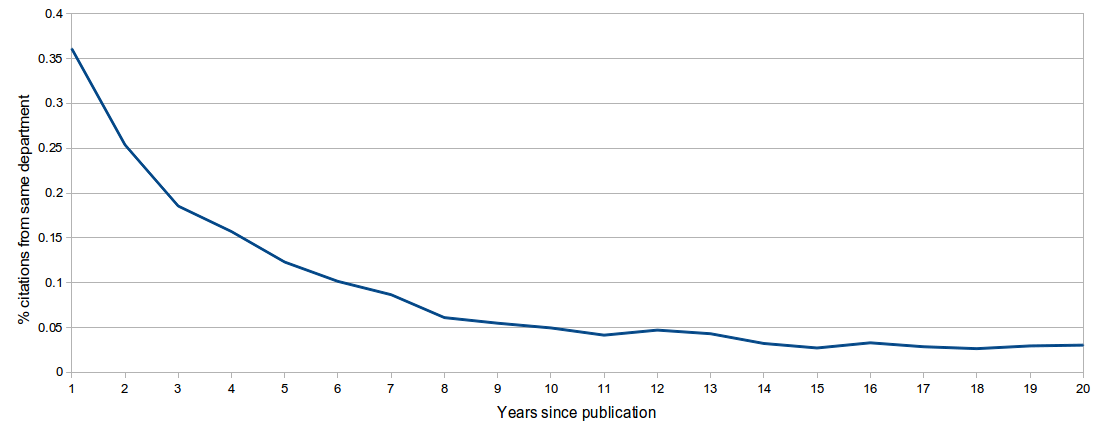
\includegraphics[scale=0.35]{pics/raw_diffusion.png}
    \caption{Citing paper location sharing over time.}
    \label{fig:rawdiffusion}
\end{figure}

In what follows, I will describe the main model, then discuss data and
estimation. In the estimation section I will discuss the identification
strategy, describe the source of exogenous variation, and discuss the
actual implementation of the estimation routines. Following that is a
results section, and a counterfactual section, and the cross-country calibration.
Penultimately, several alternative
specifications are estimated, and the models are simulated and checked
against data.  Finally, the results of a reduced-form probit model with a similar 
message to the main structural model are presented.

\section{An Empirical Model of Knowledge Diffusion}
\label{sec:model}

\subsection{Learning and Citation}
\label{sec:learncit}

Time is discrete. There is a finite number $A$ of academics partitioned
at any particular time into $D$ departments. Each academic is endowed with a quality
$q_i$ and either the same field as the new paper ($f_i = 1$) or another
field ($f_i = 0$). Each academic also has an unobserved latent type
$h_i \sim \mathcal{N}(0,\sigma^2)$, which captures his field-specific
skill in discovering new research.

At time $0$ a new paper
is written in a particular field.  If an academic is \emph{potentially interested} in the
paper, he is susceptible to learning about its existence.
I assume that potential interest in a paper is independently drawn once for each
academic from a Bernoulli distribution with success probability dependent upon field $f_i$: 
$\gamma_{f_i} \in \{\gamma_0, \gamma_1\}$.
The probability of a potentially interested academic learning about the paper
depends on the fraction of
other academics in his department who have already learned about the paper,
his observable characteristics, and his unobserved latent type. Upon
learning about the paper, an interested academic immediately cites it.\footnotemark\footnotetext{There is an extension in Section \ref{sec:extensions} in which the model is estimated with a deterministic one-year publication lag.  If we are willing to additionally assume that an academic can not transfer knowledge until he actually publishes something citing the new paper, it would be feasible to make publication lags random as well.}

More formally, the probability that a potentially interested
academic who has not yet learned
about a paper learns about it at time $t$ is given by the
logit:\footnotemark\footnotetext{At first glance, this looks like the typical dynamic logit, but it is simpler.  A dynamic logit has state dependence.  The econometrician needs to estimate the extent that the outcome today depends on the outcome yesterday.  In the model here, once an academic learns about a paper, he needs not learn about it a second time.  Learning about a paper is like contracting a chronic disease -- one time is enough.}

\begin{equation}
    \frac{e^{\alpha + \beta K(d,t-1) + h_i}}{1 + e^{\alpha + \beta K(d,t-1) + h_i}}
    \label{eq:citprob}
\end{equation}

$K(d,t-1)$ is the percentage of current colleagues who cited the
paper by $t-1$. Equation \eqref{eq:citprob} is the only place in the
model where $\beta$, the main parameter of interest, appears. The
parameter $\beta$ measures the direct effect of the knowledge of colleagues on own
learning. The latent type $h_i$ can either increase or decrease the
probability of citing, depending on its sign.

\subsection{Dynamic Department Choice Problem}

In this section, I develop a model of labor movement between departments.  It is necessary to model movement because the counterfactual exercises we are interested in involve changing mobility among departments.  Explicitly modeling movement disciplines the way that movement patterns change when mobility is increased.  In addition, treating moves as random would bias the estimates of the learning and citing parameters in Section \ref{sec:learncit}.\footnotemark\footnotetext{An alternative reduced-form method to deal with bias is to use an instrumental variables approach.  This is done in Section \ref{sec:end_probit}.}

%reset footnote counter
\setcounter{footnote}{0}

In the model, an academic decides in which department to work in order to
maximize discounted lifetime expected utility. If the academic chooses to move, he must pay a movement cost.  The model is a dynamic discrete choice model, similar in spirit to recent work by \citet{kennan2011effect} on interstate migration.\footnotemark\footnotetext{Since knowledge diffusion is the main focus of this paper, for tractability the location choice model developed here is simpler than that in Kennan and Walker.  In particular, I assume that movement costs are the same for all department pairs.  \citet{dahl2002mobility} is an alternative for estimating the migration decision between many possible locations.  In the Dahl model, however, migration decisions are taken only once in the lifetime of a worker.  Since my data contains repeated migration observations,  a version of the dynamic Kennan and Walker model is more appropriate.} Department choice is the only decision in the model.

Let $\mathbf{X}_i$ be the vector of personal characteristics of academic $i$: field $f_i$, quality
$q_i$, and latent type $h_i$. If academic $i$ works at department
$d$ in period $t$, he gets period random utility:

\begin{equation}
    u_{i,t}(d) = W(d, \mathbf{X}_i) + \varepsilon_{i,d,t}
    \label{eq:util}
\end{equation}

Period utility is a department-specific, time-invariant payoff, plus a time-varying preference shock.  The preference shock
 $\varepsilon_{i,d,t}$ is distributed IID Type 1 Extreme Value.
The current-period payoff to working at department $d$ can be split into two parts:

\begin{equation}
    W(d, \mathbf{X}_i) = w_v(\mathbf{X}_i) + w(d, \mathbf{X}_i)
\end{equation}

The first part of the period payoff $w_v$ depends only
on personal characteristics like quality and field. This component is the 
same at any department.  The second part of the payoff
$w$ is department specific. It depends on time-invariant measure of department
field $F_d$, and time-invariant measure of department quality $Q_d$, both of which interact with
individual field, quality, and latent type.\footnotemark\footnotetext{In practice, department 
field is the mean annual fraction of academics in the field working at the department.  Academic 
quality will be lifetime mean citations per paper, and department quality is the mean 
annual average quality of academics working at the department
during the sample period.  Details are contained in Section \ref{sec:dat}.}:

\begin{equation}
    \ln w(d, \mathbf{X}_i) = \xi_0  + \xi_q q_i Q_d + \xi_f f_i F_d + \xi_h h_i F_d
    \label{eq:horz_wage}
\end{equation} 

Latent type $h_i$ is interacted with department field $F_d$ because those with high
skill in discovering new research value having colleagues
in the same field differently than those with low skill.

Movement costs $\mathcal{C}$ must be paid each time an academic changes departments.\footnotemark\footnotetext{In principle, movement costs could depend on interactions between department and the observable characteristics in the payoff equation, with some exclusion for identification.  The current specification forces all sorting to go through interactions in the payoff equation.  I suspect that substitution patterns would not be much more rich in a specification with characteristic-dependent movement costs, so to save parameters I estimate the simpler model.} Saving is not allowed. Agents choose departments to maximize discounted lifetime expected utility.
The value function below is net of the non-department-specific payoff component $w_v$.\footnotemark\footnotetext{In particular, if we add $\frac{\rho}{1 - \rho} w_v$ to the left hand side of \eqref{eq:val_fun}, and add $w_v + \frac{\rho}{1 - \rho} w_v$ to every appearance of $V(.)$ on the right hand side, the new terms cancel out and the equation remains the same.}
The set of departments is $\mathcal{D}$.
Suppress the permanent characteristic vectors $\mathbf{X}_i$ and write the
recursive value function as:

\begin{align}
    V(d) &= \rho \mathbb{E}_\varepsilon \big[\max\{V(d') + w(d') + \varepsilon_{i,d',t} - \mathbbm{1}_{\{d'\neq d\}} \ \mathcal{C}\}_{d'\in \mathcal{D}}\big] \nonumber \\
    &= \rho \gamma_e + \rho \ln\left( \sum_{d' \in \mathcal{D}} e^{V(d') + w(d') - \mathbbm{1}_{\{d'\neq d\}} \ \mathcal{C}} \right)
    \label{eq:val_fun}
\end{align}

The substitution of the expectation of the maximum of Type I Extreme Value errors
in \eqref{eq:val_fun} follows \citet{rust1987optimal}, and is derived in Appendix \ref{sec:exp_der}. This value function
 is defined on $D$ departments for each type $\mathbf{X}_i$, with $\gamma_e \approx 0.577$ being the Euler-Mascheroni constant. I
show in Appendix \ref{sec:contr_map} that the natural operator on \eqref{eq:val_fun} is a
contraction mapping. We can use the value function to get the
probability of moving from department $d$ to another department $d'$:

\begin{equation}
    Pr(d,d') = \frac{e^{V(d') + w(d') - \mathbbm{1}_{\{d'\neq d\}}\mathcal{C}}}{\sum_{d'' \in \mathcal{D}} e^{V(d'') + w(d'') - \mathbbm{1}_{\{d''\neq d\}} \mathcal{C}}}
    \label{eq:trans}
\end{equation}

\subsection{Summary} 

The model can be thought of as consisting of two parts.  The learning and citing part is 
a stochastic process governed by \eqref{eq:citprob}.  Only the observable department 
citation fraction $K(d,t-1)$ varies over time.\footnotemark\footnotetext{See Section \ref{sec:extensions} for an extension 
in which there is a national knowledge spillover as well.}
The part of the model governing movement between firms is a dynamic discrete
choice problem, characterized by the value
function \eqref{eq:val_fun} and the utility function \eqref{eq:util}.
 Solving the value function results in transition probabilities
 which depend on fixed observable and unobservable characteristics.  The link between the two parts
 of the model is the latent type $h_i$, which affects both
payoffs and learning probabilities.  While latent type is unobserved, it is assumed
to be fixed over time.  This extreme form of serial correlation
 will be discussed further in Section \ref{sec:ident}.

\subsection{Initial Conditions}
\label{sec:init_cond}

In the model described above, latent type $h_i$ is assumed to be
independently randomly distributed. There is, however, an interaction in
payoffs between unobserved latent type and department field.
This interaction will induce sorting before my sample period, so if I
take latent type to be randomly distributed I will get inconsistent
estimates. Put simply, an academic is more likely to be of high latent type if he is
first observed at a department with a high fraction of workers in the field of
the new paper. To mitigate this
problem, I assume that the mean of the distribution of latent
type depends upon the department observed in an academic's first year.  Here $F^{(1)}_i$ denotes the 
field fraction and $Q^{(1)}_i$ the quality of the observed first department of academic $i$:

\begin{equation}
    h_i = \phi_Q Q^{(1)}_i + \phi_F F^{(1)}_i + h^*_i, \ \ \ \ \  h^*_i \sim \mathcal{N}(0, \sigma^2)
    \label{eq:initcond}
\end{equation}

Any level effect in \eqref{eq:initcond} will be absorbed by $\alpha$ in the learning probability equation \eqref{eq:citprob}, and the size of parameter $\xi_l$ in period payoff equation \eqref{eq:horz_wage}. The quantities $F^{(1)}_i$ and $Q^{(1)}_i$ depend only on the \emph{initial} observed
department of an academic, while the department field $F_d$ and quality $Q_d$ entering
into \eqref{eq:horz_wage} depend on the current location of the academic which may change from year to year.

\subsection{Likelihoods}

My data describe a set of academic economists over time, and the citations of a particular paper over time.  For academic $i$, the key variables are the (possibly empty) year of academic $i$'s first citation
of the new paper $C_i \in 1,2,\dots, T \cup \emptyset$, and a (possibly empty) department for academic $i$ in each year $M_{i,t}$.  Collect into sets $\mathbf{C} = \{C_i\}_{i \in A}$,
$\mathbf{M} = \{M_{i,t}\}_{i \in A, t \in 1,\dots, T}$, and $\mathbf{M}_i = \{M_{i,t}\}_{t \in 1,\dots, T}$. 
 As before, let $\mathbf{X}_i$ be all individual characteristics, both observable and unobservable.  Let $\mathbf{X}_{o,i}$ denote only
 observable individual characteristics, and let $\mathbf{X}_o = \{\mathbf{X}_{o,i}\}_{i\in A}$. Let $H$ denote
the mean-zero normal CDF with variance $\sigma^2$, i.e. the distribution
of $h^*_i$ as in \eqref{eq:initcond}.  Let $\mathfrak{D}$ be the set of departments.  Department fields $F_d$ and qualities $Q_d$ are 
contained in the vector $\mathbf{Z} = \{F_d, Q_d\}_{d \in \mathfrak{D}}$. Suppose
that we have calculated the transitions $Pr(d,d'\vert \mathbf{X}_i, \mathbf{Z}, \theta)$ from
value function iteration. We can consider the likelihood for each
individual separately. The likelihood for academic $i$ is:

\begin{align}
    Pr(C_i,\mathbf{M}_i|\mathbf{X}_{o,i},\mathbf{Z},\theta) &= \int Pr(C_i,\mathbf{M}_i|h_i, \mathbf{X}_{o,i},\mathbf{Z},\theta) dH \nonumber \\
    &= \int Pr(C_i,\mathbf{M}_i|\mathbf{X}_i,\mathbf{Z},\theta) dH
    \label{eq:inth}
\end{align}

We can split the integrand in \eqref{eq:inth} into multiplicative terms:

\begin{equation}
    Pr(C_i,\mathbf{M}_i|\mathbf{X}_i,\mathbf{Z}, \theta) = Pr(C_i|\mathbf{X}_i, \mathbf{M}_i, \theta) Pr(\mathbf{M}_i|\mathbf{X}_i, \mathbf{Z}, \theta)
\end{equation}

The second part comes directly from the transitions derived from the
value function iteration.  We construct it by multiplying probabilities of observed
moves:\footnotemark\footnotetext{Entry and exit are treated as exogenous.  If $M_{i,t} = \emptyset$ or $M_{i,t+1} = \emptyset$, then $Pr(M_{i,t}, M_{i,t+1}\vert \mathbf{X}_i, \mathbf{Z}, \theta) = 1$.}

\begin{equation}
    Pr(\mathbf{M}_i|\mathbf{X}_i,\mathbf{Z},\theta) = \prod_{t = 1}^{T-1} Pr(M_{i,t}, M_{i,t+1}\vert \mathbf{X}_i, \mathbf{Z}, \theta)
    \label{eq:mov_liks}
\end{equation}

The first part is a little more complicated. Set $M_{i,0} = \emptyset$ for notational convenience:

\begin{align}
    &Pr(C_i|\mathbf{X}_i, \mathbf{M}_i, \theta) = \left[\left(1 - \gamma_{f_{i}}\right) + \gamma_{f_{i}} \prod_{t=1}^T \left(1 - 1_{\{M_{i,t}\neq \emptyset\}} \frac{e^{\alpha + \beta K(M_{i,t},t-1) + h_i}}{1 + e^{\alpha + \beta K(M_{i,t},t-1) + h_i}}\right)\right]^{1_{\{C_i = \emptyset\}}} \nonumber \\
    &\times \left[\gamma_{f_{i}} \prod_{t=0}^{C_i - 1} \left(1 - 1_{\{M_{i,t}\neq \emptyset\}} \frac{e^{\alpha + \beta K(M_{i,t},t-1) + h_i}}{1 + e^{\alpha + \beta K(M_{i,t},t-1) + h_i}}\right) \frac{e^{\alpha + \beta K(M_{i,C_i},C_i-1) + h_i}}{1 + e^{\alpha + \beta K(M_{i,C_i},C_i-1) + h_i}}\right]^{1_{\{C_i \neq \emptyset\}}}
    \label{eq:cit_lik}
\end{align}

The two big multiplied terms in \eqref{eq:cit_lik} reflect the
difference between those I observe citing the paper and those I do not.
If I observe that an academic cited the paper ($C_i \neq \emptyset$), he must have been
interested in it. If the academic didn't cite the paper ($C_i = \emptyset$), then either he was not
interested, or he would have been interested but did not hear about the paper during 
the years in my data. In the top term, the $(1 - \gamma_{f_i})$ is the probability $\gamma_{f_i}$
that the academic was not interested. The second term on the top line is the probability that
the academic would have been interested had he heard about the paper,
multiplied by the probability that he did not hear about the paper.  The indicator function $1_{\{M_{i,t}\neq \emptyset\}}$
eliminates years when an academic is not in the data set.  The bottom line is
simply the probability that an academic was interested $\gamma_{f_i}$ multiplied
by the probability that the academic did not hear about the paper until
the year he did, and then multiplied by the probability that he did hear
about the paper in the year he cited it.

Combining all the academics, the total likelihood is then:

\begin{equation}
    Pr(\mathbf{C},\mathbf{M}|\mathbf{X}_o,\mathbf{Z},\theta) = \prod_i Pr(C_i,\mathbf{M}_i|\mathbf{X}_{o,i}, \mathbf{Z}, \theta)
    \label{eq:fulllik}
\end{equation}

\section{Data Description}
\label{sec:dat}

\subsection{General Data Construction}

In this section I describe with some generality how the data used in all
exercises in this paper were collected and constructed.  Section
\ref{sec:struct_dat} describes the specific construction of variables
used in the estimation of the structural model described above.

An academic's current place of employment is listed under the byline on
academic papers. The Thomson-Reuters Web of Knowledge, a citation
database, records affiliation for each academic on each available paper. I use the
python web scraping library BeautifulSoup to download citation data for
more than one hundred thousand economics articles from the Web of
Knowledge, and then use affiliation data to construct a panel of
economists moving between departments. Recent independent research by
\citet{agrawal2013why} constructs a similar panel of academics also from
Thomson-Reuters Web of Knowledge, but uses evolutionary biologists rather than economists.

I describe how the data was cleaned and filtered in
Appendix \ref{sec:dat_cons}. In addition to direct information on each economics paper, I
also collected data on all papers from any discipline which cite either the
most cited hundred economics papers, or that cite any economics paper
published in 1980 or 2005.\footnotemark\footnotetext{In another project using this data, I am looking at the 
    effect of the internet on diffusion rates.  I choose 1980 because it is well before the internet era, 
and 2005 because it is well after.}  This is a large, rich data set, containing thousands
of economists, hundreds of departments from around the world, and more than 
one hundred thousand papers and citation records.

In several exercises I use the field of an economist. I
construct a field for each economist using data from IDEAS, based on
which curated mailing lists the work of an academic is mainly distributed in. 
This way of classifying field is not original to me -- it is currently
an experimental classification system on IDEAS itself.

An economist can simultaneously work in many areas.  What I will refer to as a 
field is a 91-dimensional unit vector describing research area. This is a 
fine disaggregation scheme.  For instance, someone doing trade and operations research
will correctly have a different field vector from someone doing trade and public economics. 
If the work of an economist is distributed in the IDEAS development 
mailing list as well as the game theory mailing list, he will
have a field vector of 89 zeros, with $\frac{1}{\sqrt{2}}$ in the
dimensions corresponding to game theory and development. 

Journal fields are constructed using the JEL field rankings in \citet{barrett2000subdiscipline}.
To get a field for each paper, journal and academic fields are combined and normalized.
Field construction is described in detail in the data appendix, Appendix \ref{sec:dat_cons}.

\subsection{Baseline Structural Model}
\label{sec:struct_dat}

In this section I describe the construction of variables specific to the estimation
of the structural model described in Section \ref{sec:model}.  The model is
estimated using first citation
times of a single paper: Michael Jensen's 1986 \emph{American Economic
Review} piece ``Agency costs of free cash
flow, corporate finance, and takeovers''.
Estimating the structural model on
citations of a single paper allows me to use a binary field,
which greatly reduces the complexity of the department choice problem.
I can also focus on data from a relatively small number of years around the time the paper
was published.  Finally, using a single paper allows me to keep the parameter 
space small.  Papers have widely varying citation trajectories, and most
papers have very few citations.  If we were to include many papers in the model,
we would need to let the potential interest parameters  $\gamma_0$ and $\gamma_1$
vary across papers, leading to a large parameter space and imprecise estimates.\footnotemark\footnotetext{
    As a robustness check, I reestimate the entire model using \citet{grossman1986costs},
    another influential paper published in 1986.  In Appendix \ref{sec:gross} I present a comparison of the reestimated results
 to the baseline results, and find essentially no difference.}

Jensen's 1986 \emph{American Economic Review} piece is one of the most highly
cited papers in my data set, giving me many observations of citation
times. The paper was published just before Jensen ended his joint
appointment with the University of Rochester where he spent the first 20
years of his career, and permanently moved to the Harvard Business
School. I use the Jensen paper because most of the other highly cited papers 
are in the field of econometrics. The most highly cited econometrics papers are those 
which become widely used by applied economists.  For example, two of the most cited
papers in my dataset are \citet{heckman1979sample} and \citet{white1980heteroskedasticity}.
 For these papers, field is a poor measure of interest.  The Jensen paper, on the
 other hand, is still more likely to be cited by economists working in contract theory or business
economics.

The binary academic specific
field $f_i$ is set to one if an academic works in
either of the Jensen fields: ``Contract Theory and Applications'' or ``Business Economics''.
The department field $F_d$ is the mean fraction of academics in the department in the 
Jensen field, averaged over all years in my sample.  To create the quality of an academic, I
first calculate his mean coauthor-adjusted lifetime citations per published paper. To reduce the
dimensionality of the problem, I then partition academics into equally-sized
low and high quality groups.\footnotemark\footnotetext{One can imagine
several ways to measure the quality of an academic based on publications and citations.
One alternative would be a simple count of published papers per year.  Another would be
total citations per year.  While the choice of quality metric will change the
ranking of academics to some degree, I believe different metrics will lead to
similar aggregated high and low quality groups.}  I assign the high-quality group $q_i = 1$, 
and the low quality group $q_i = 0$.  Department quality $Q_d$ is based on the REPEC ranking
of US departments, with departments assigned equally spaced values of $Q_d \in [0,1]$.

I use data from the 104 American departments ranked in the top 25\% of
US departments by REPEC. Data from lower-ranked departments is
available, but noisy because, economists at low ranked departments
publish relatively rarely. I observe the location of an economist
only when his work appears in a journal. To give some idea about what is
excluded, the three lowest ranked included universities are Clark
University, the Georgia Institute of Technology, and the University of
New Mexico. I drop all economists who never worked at any of the 104 departments 
in my dataset.  If an economist in my dataset spent some years at a
department not included, I classify his department in those years as
``other''. I estimate the model on data for the eight years beginning
in 1987, the year after Jensen's paper was published. Tables \ref{tab:aut_sum}
and \ref{tab:dep_sum} contain summary statistics for the data I use in
estimation.

\begin{table}[!ht]
    \centering
    \begin{tabular}{lllllll}
        \hline \hline
              \    & Obs Number & In Field & Citers & Moves & Cits / Pap, avg & Cits / Pap, sd \\ \hline 
        Academicss  & 3876       & 150      & 122    & 679   & 26              & 29             \\ \hline
    \end{tabular}
    \caption{Academic summary statistics}
    \label{tab:aut_sum}
\end{table}

\begin{table}[!ht]
    \centering
    \begin{tabular}{lllllll}
        \hline\hline
                    & Obs Number & 1987 med size & 1994 med size & Field, (avg, sd) & Avg cits / pap, (avg, sd) \\ \hline
        Departments & 104        & 16               & 24               & (0.03,0.06)           & (20,9) \\ \hline
    \end{tabular}
    \caption{Department summary statistics}
    \label{tab:dep_sum}
\end{table}

\section{Identification and Estimation Routine}

\subsection{Identification and Causality}
\label{sec:ident}

The main parameter of interest is $\beta$ in \eqref{eq:citprob}, the
impact of colleagues on own learning about new ideas. It
governs not only peer-learning directly, but it also reflects the importance 
of movement between departments.  A high $\beta$ implies that a knowledgeable
colleague makes an academic much more likely to learn about the new paper.

The three common peer effect identification challenges are endogenous sorting,
correlated effects, and the reflection problem.  The peer effect in my
model works with a lag, that is citation probabilities are affected only by 
lagged colleague knowledge.  There is a clear direction of 
causality implied by time, so the reflection problem is not an issue.

Endogenous sorting and correlated shocks remain a challenge.  Academics might sort into 
departments based on unobservables. An academic may cite
earlier because his colleagues have already learned about a paper, or it
could could just be that he is working with people interested in
similar things. Even if he had been at a different department, he would
have been among the early citers.

%reset footnote counter
\setcounter{footnote}{0}

The model developed above allows the citing probability to be influenced
by unobserved fixed individual characteristics $h_i$, and allows for
sorting on these unobserved characteristics. Even if academics sort into
departments based on time-invariant unobservables, identification is
possible using moves between departments and time series variation. For
example, suppose that an academic who has cited the Jensen paper moves from
Cornell to Penn State. I can observe citing behavior at Penn State
before the academic arrives, and
citing behavior at Cornell after he leaves. If all characteristics of
Penn State and Cornell academics are fixed, then the change in citing
behavior can be used to infer $\beta$. In the language of an experiment,
the control group is Penn State academics just before the new colleague
arrives, and the treatment group is Penn State academics after the
colleague arrives.  As mentioned in the introduction, the assumption that 
 fixed effects are time-invariant is common in the structural spillover literature,
 especially the non-experimental labor literature on peer
 effects in school classrooms.\citep{bettsa2004peer, arcidiacono2012estimating, burke2013classroom}\footnotemark\footnotetext{
There is an even larger labor literature on the value-added
effect of teachers on student achievement.  This literature also needs
to deal with endogenous sorting, and uses student fixed effects when
possible (see \citet{harris2011teacher} for a recent example).
In this context, \citet{rothstein2010teacher}
finds evidence that student fixed effects are not sufficient to control
for endogenous sorting.}

What is not in the model is serially-correlated, time-varying unobserved
individual or correlated shocks. If such persistent time varying shocks cause a group of people to
sort together and subsequently begin citing each other papers, the
baseline structural model will overestimate learning from colleagues.
In the current setting, however, ignoring serially correlated shocks is 
unlikely to seriously bias the estimates.  While research interests can
change over the lifetime of an academic, there is a strong lock-in effect
due to the high fixed costs of reaching the research frontier in an unfamiliar
area.  Substantial change in research focus takes place at most
several times in a career, and the model is estimated on only eight
years of data.

If serially correlated shocks were important, however, to identify the
causal effect of coworkers on learning one would need an exogenous shock
which affects the location choice of an academic, but does not affect
citations.  I use the US recession of 1990-1991 to induce exogenous
movement. Some states were hit particularly hard by the crisis, and some
state schools were forced to implement temporary hiring freezes. I will
argue that these hiring decisions by state schools in 1991 induced
exogenous changes in movement patterns between departments, but did not
affect citing behavior.

In the baseline structural model, I include the shocks as a temporary
source of variation in payoff. I describe how I do this in detail
in the next section.  I also run an endogenous probit, using state budget
deficits as an instrument, with the exogeneity assumption that the 1991
recession affected movement choices but did not affect citing behavior.\footnotemark\footnotetext{
There is also a quasi-experimental labor literature
 on peer-effects in the classroom employing instrumental variable 
methods to deal with endogenous sorting and other identification issues.
\citep{kang2007classroom, de2010identification}}
The estimated coefficient on $\beta$ in the reduced-form instrumental variable
exercise is similar in size to the estimate in the structural 
estimation.

As for the other parameters, first consider the citing probability
$\eqref{eq:citprob}$. The variance in citing frequencies net of the
$\beta$ coworker effect will identify the dispersion of latent type, and
the level of citation frequencies net of $\beta$ identifies $\alpha$.
Since the dispersion of latent type is identified from
$\eqref{eq:citprob}$, the parameter $\xi_h$ along with the other payoff
parameters $\xi$ are identified by observed department move choices in the data, i.e.
substitution patterns. The cost of movement $\mathcal{C}$ is
identified by the frequency of moves.

\subsection{Exogenous Variation: Economic Malaise of 1990-1991}

Induced partly by an oil price shock caused by the Iraqi invasion of
Kuwait, the United States went through an economic recession from July,
1990 to March, 1991. The effects of the downturn differed by state.
\citep{wapo1991public, moore1991state} In several of the hardest hit
states, public universities implemented hiring freezes for various
lengths of time.\citep{latimes1991golden, moneymag1991paying, uvt2013pres}
I use data on state budget deficits in fiscal year 1991 to proxy for
temporary, unanticipated hiring reductions at public universities in
1991.\citep{gold1995fiscal}

 Let $b_d$ be the 1991 budget deficit
divided by total state expenditures in the state of public university
$d$.   Several linear regressions show that the 1991 economic downturn induced observable variation
in movement patterns.  The unit of observation is a department-year, and the dependent variable
 is net moves into a department.  The independent variable we care about is dum91bd, a 1991
dummy multiplied by budget shortfall $b_d$. The regression is performed
on 104 departments with seven years of observation starting in 1986, which
is similar to the data cut I use in the structural exercise.
 Table \ref{tab:bd_reg} reports results.

\begin{table}[h]
    \centering
    \begin{tabular}{lllll}
        \hline\hline
                            & net in-moves &   net in-moves &     net in-moves &    net in-moves \\   \hline 
dum91bd                     &     -8.568** &     -12.280**  &      -6.784**    &      -7.055**   \\
                            &      (4.24)  &      (4.93)    &      (2.88)      &      (2.84)     \\
year dummies                &        no    &         yes    &          yes     &         yes     \\
dep dummies                 &        no    &         no     &          yes     &         yes     \\
dep dummies $\times$ year   & no           &  no            &   no             &  yes            \\  \hline
Obs                         & 617          &  617           &   617            &  617            \\
$R^2$                       & 0.01         &  0.02          &   0.77           &  0.82           \\  \hline
    \end{tabular}
    \caption{The net in-move effect of state budget shortfalls}
    \label{tab:bd_reg}
\end{table}

Some states had 1991 budget deficits $b_d$ as large as $15$ and $20\%$, implying
one to two fewer net in-moves into public universities compared with a typical year.

In the structural model, I make use of the shock to state budgets by assuming that in 1991 payoffs
 (wages) are suddenly and temporarily shocked so that:

\begin{equation}
    w_{1991}(d, \mathbf{X}_i) = e^{- \xi_{ex} b_d p_d} w(d, \mathbf{X}_i)
    \label{eq:exog_var}
\end{equation}

Here $p_d$ is a dummy set to $1$ if $d$ is a public university.  Since this payoff
cut is sudden and temporary, it does not affect
expectations in the value function.  What this means for the estimation is that
for the single year 1991 transition probabilities between departments 
in the movement likelihood \eqref{eq:mov_liks} are given by \eqref{eq:1991trans} rather than
the original transition probabilities \eqref{eq:trans}.\footnotemark\footnotetext{See Section \ref{sec:end_probit} for an alternative
reduced-form analysis using 1991 budget deficits as an instrument.}

\begin{equation}
    Pr_{1991}(d,d') = \frac{e^{V(d') + w_{1991}(d') - \mathbbm{1}_{\{d'\neq d\}}\mathcal{C}}}{\sum_{d'' \in \mathcal{D}} e^{V(d'') + w_{1991}(d'') - \mathbbm{1}_{\{d''\neq d\}} \mathcal{C}}}
    \label{eq:1991trans}
\end{equation}

\subsection{Implementation}

I estimate the twelve parameters in the likelihood function \eqref{eq:fulllik}
using Bayesian inference and Markov Chain Monte Carlo (MCMC).  Description of the priors
are contained in Table \ref{tab:priors}.  The priors are mostly designed to be proper but 
relatively uninformative.  For parameters which a priori fall anywhere on the real line
I use the normal distribution centered at zero with variance 100, and for parameters which
are a priori non-negative I use the exponential distribution with parameter 300.\footnotemark\footnotetext{The exponential prior has 
been used for a similar purpose in the epidemiology literature.\citep{cauchemez2004bayesian}  In earlier 
versions of the paper I used mostly improper diffuse priors (for parameters including the peer effect $\beta$) and ended up with very similar posteriors in the baseline model.  Appendix \ref{sec:prior_comp} compares the baseline model with an estimated version in which $\beta$'s prior is diffuse and finds almost no qualitative difference.  In the model extensions, some results are sensitive to the choice of prior, in particular the version in which I allow all parameters in the knowledge diffusion process to depend upon observed field.  There are too few people in Jensen's field to provide strong evidence on so many parameters.  Since there are theoretical reasons to expect that colleague knowledge should not cause less learning, I use the exponential prior for all peer effects.}
There are weakly informative priors are on the interest parameters $\gamma$ because I can
observe whether the academics in my eight-year sample cited the Jensen paper anytime up to
2012. If an academic has not cited the influential Jensen paper 25 years after it was
published, it is probably not because he has yet to hear about it.
About a third of people in Jensen's field ultimately cite the paper, so I assign a beta
distribution with parameters 1 and 2 to the field interest probability
$\gamma_1$. The standard deviation of the prior is 0.24. About 6\% of
people not in the field ultimately cite the paper, so I assign to the
non-field interest probability $\gamma_0$ a beta distribution with
parameters 1/8 and 2, which gives a standard deviation of 0.13.

\begin{table}[!ht]
    \centering
    \begin{tabular}{ll}
        \hline\hline
                             & \textbf{Prior} \\ \hline
         $\alpha$            & Norm(0,100)    \\ 
         $\beta$             & Exp(300)       \\ 
         $\gamma_{F}$        & Beta(1,2)      \\ 
         $\gamma_{NF}$       & Beta(0.125,2)  \\ 
         $\xi_f$             & Norm(0,100)    \\ 
         $\xi_l$             & Norm(0,100)    \\ 
         $\xi_q$             & Norm(0,100)    \\ 
         $\mathcal{C}$       & Exp(300)       \\ 
         $\phi_F$            & Norm(0,100)    \\ 
         $\phi_Q$            & Norm(0,100)    \\ 
         $\sigma$            & Exp(300)       \\ 
         $\xi_{ex}$          & Exp(300)       \\ \hline

    \end{tabular}
    \caption{Priors}
    \label{tab:priors}
\end{table}

Recall that I partition academics into two quality groups,
field is binary, and I use four
points to approximate the one-dimensional numerical integral over $h_i$.
Thus, in each iteration of the estimation routine there are 16 independent value
functions to solve, each on a space of 104 departments.

The MCMC employed for the estimation is a random walk Metropolis
algorithm with an adaptive proposal distribution. The art in MCMC is choosing
efficient proposals. In
the plain random-walk metropolis method, a proposal is just mean-zero Gaussian
random noise $\epsilon$ added to the current parameter set. It is difficult
to determine an efficient covariance
structure for $\epsilon$ a priori. If the jumps are large or in unlikely
directions, then the proposal is accepted too rarely and it takes a
long time to move around the posterior. On the other hand, if jumps are
too small, then the proposal is almost always accepted and the routine
must be run a long time to spend enough time in the high probability
areas of posterior distribution.

To get an efficient covariance structure, I employ the adaptive
algorithm suggested by \citet{haario2001adaptive}. In every step of the
algorithm the empirical covariance structure of many previously accepted
parameters is calculated. The random noise for the next proposal is then
drawn from a mean-zero Gaussian distribution with the calculated
empirical covariance structure. \citet{haario2001adaptive} show that
this algorithm will asymptotically approach the efficient covariance
structure. Parameters are updated block by block, with only a single
block being updated in each step. There are three blocks: parameters
related to learning and citing ($\{\alpha,\beta,\gamma\}$), parameters
related to moving ($\{\xi,\psi,\lambda_o\}$), and latent type parameters
($\{\phi,\sigma\}$). The covariance structures are updated for each of
the parameter blocks separately.

The MCMC routine is implemented in python 2.71, making heavy use of the
excellent pandas (panel data analysis) library as well as
the python multiprocessing library. Each time I estimate the model, I ran 10 separate
chains using Penn State Research Computing resources.
The first half of each chain is discarded as a burn-in.
Appendix \ref{sec:MCMC_diag} contains convergence
diagnostics for the MCMC chains as well as mixing plots. Running many
chains in parallel allows for implementation of the Gelman-Rubin
convergence criterion.\citep{gelman1992inference} Without going into detail, the criterion tests
for the similarity of the separate chains in terms of mean and
variance of each parameter. If each of the chains is `indistinguishable'
from the other chains after a burn in, then we say that draws from the
chains are independent draws from the posterior distribution. All
parameters in the estimation routine pass the Gelman-Rubin test.

\section{Analysis of Results}

\begin{figure}[!ht]
    \centering
    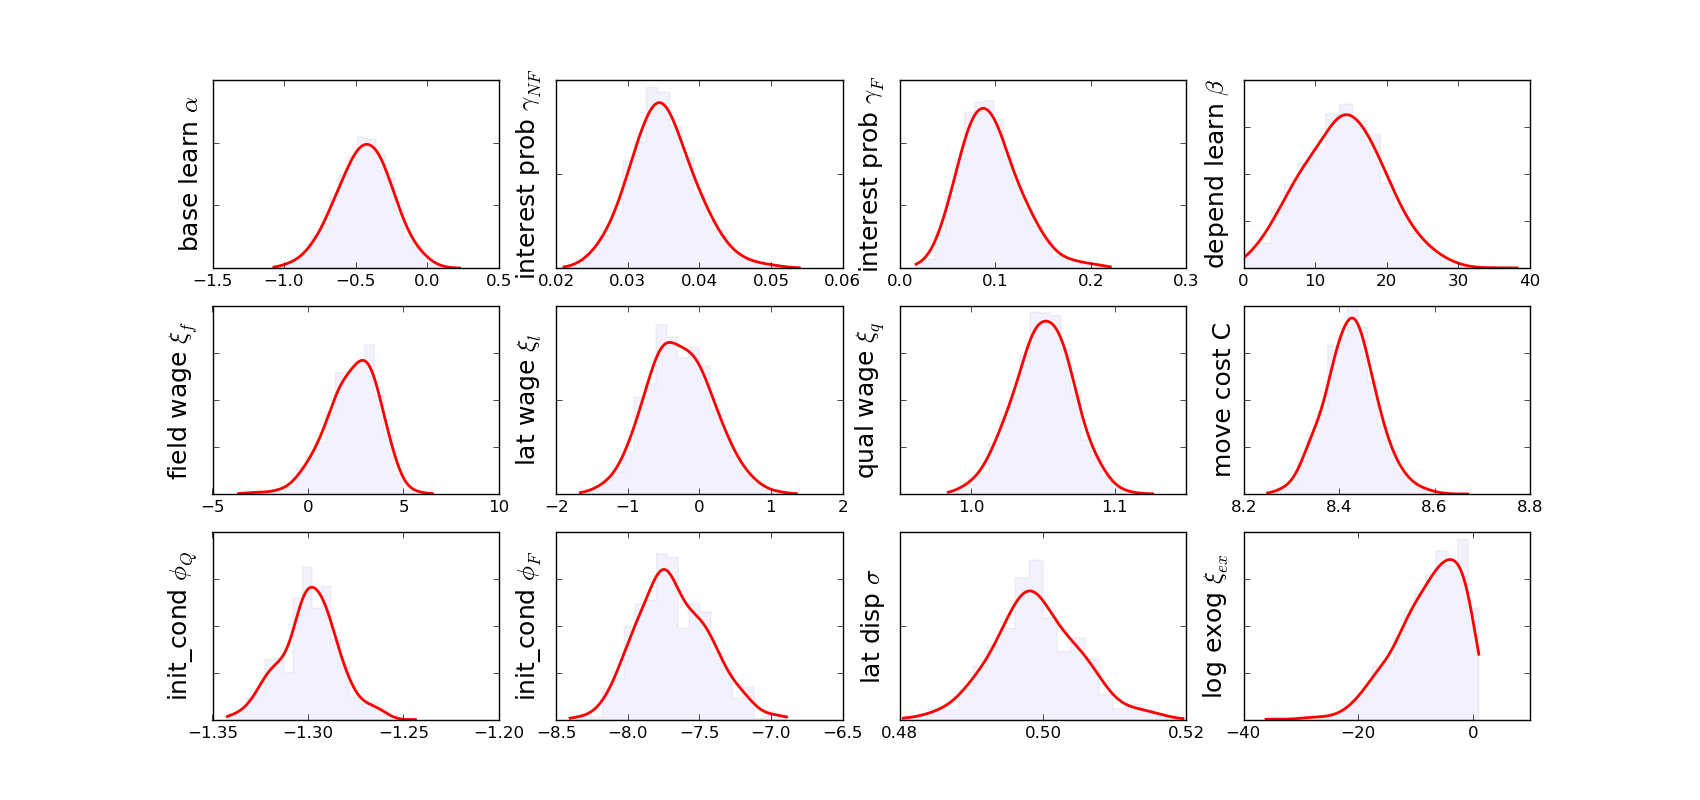
\includegraphics[scale=0.35]{pics/params_dists_big.png}
    \caption{Posterior distributions}
    \label{fig:big_params}
\end{figure}

\begin{table}[!ht]
    \centering
    \begin{tabular}{llllll}
        \hline\hline
                              & mean   & std   & 25\%   & 50\%   & 75\%   \\ \hline 
         $\alpha$             & -0.447 & 0.179 & -0.571 & -0.440 & -0.322 \\ 
         $\beta$              & 14.128 & 5.850 & 9.801  & 14.138 & 18.244 \\ 
         $\gamma_{F}$         & 0.035  & 0.004 & 0.031  & 0.034  & 0.038  \\ 
         $\gamma_{NF}$        & 0.094  & 0.031 & 0.072  & 0.092  & 0.112  \\ 
         $\xi_f$              & 2.208  & 1.374 & 1.419  & 2.367  & 3.216  \\ 
         $\xi_l$              & -0.293 & 0.411 & -0.577 & -0.289 & -0.019 \\ 
         $\xi_q$              & 1.050  & 0.021 & 1.035  & 1.049  & 1.065  \\ 
         $\mathcal{C}$        & 8.426  & 0.052 & 8.387  & 8.426  & 8.462  \\ 
         $\phi_Q$             & -1.302 & 0.014 & -1.312 & -1.302 & -1.293 \\ 
         $\phi_F$             & -7.603 & 0.230 & -7.754 & -7.611 & -7.443 \\ 
         $\sigma$             & 0.499  & 0.005 & 0.495  & 0.499  & 0.503  \\ 
         $\xi_{ex}$           & 0.919  & 0.739 & 0.343  & 0.756  & 1.312  \\ \hline
                             
    \end{tabular}
    \caption{Posterior moments}
    \label{tab:post_moms}
\end{table}

Posterior moments for the twelve estimated parameters are listed in
 Table \ref{tab:post_moms}, and parameter posterior distribution kernel densities
and histograms are plotted in Figure \ref{fig:big_params}.  The first
 row of Figure \ref{fig:big_params} contains the posterior distributions
 of the base learning parameter $\alpha$, the dependent learning parameter $\beta$, the interest
 probability $\gamma_{NF}$ of those not in Jensen's field
and $\gamma_{F}$ of those in Jensen's field. The relative magnitudes and signs of the
interest parameters are in line with what one might expect. The expected interest
probability is a little more than twice as high for academics in Jensen's
field. The main parameter of interest $\beta$ is relatively large and
positive, reflecting the importance of colleagues knowledge on own
learning.

Interpreting the magnitude of the raw citation parameters is difficult.
Figure \ref{fig:learn_probs} presents the percent change in annual learning probability
from an increase from 0\% to 5\% of colleagues knowing about a new paper.
The size of the effect depends on the latent type.  The histogram in in \ref{fig:learn_probs} shows typical latent types
in the data, which are below zero because of the initial condition equation described in Section \ref{sec:init_cond}.  For
the latent types in the data, an increase from 0\% to 5\% coworker knowledge raises annual learning probabilities by 35-60\%.

\begin{figure}[!ht]
    \centering
    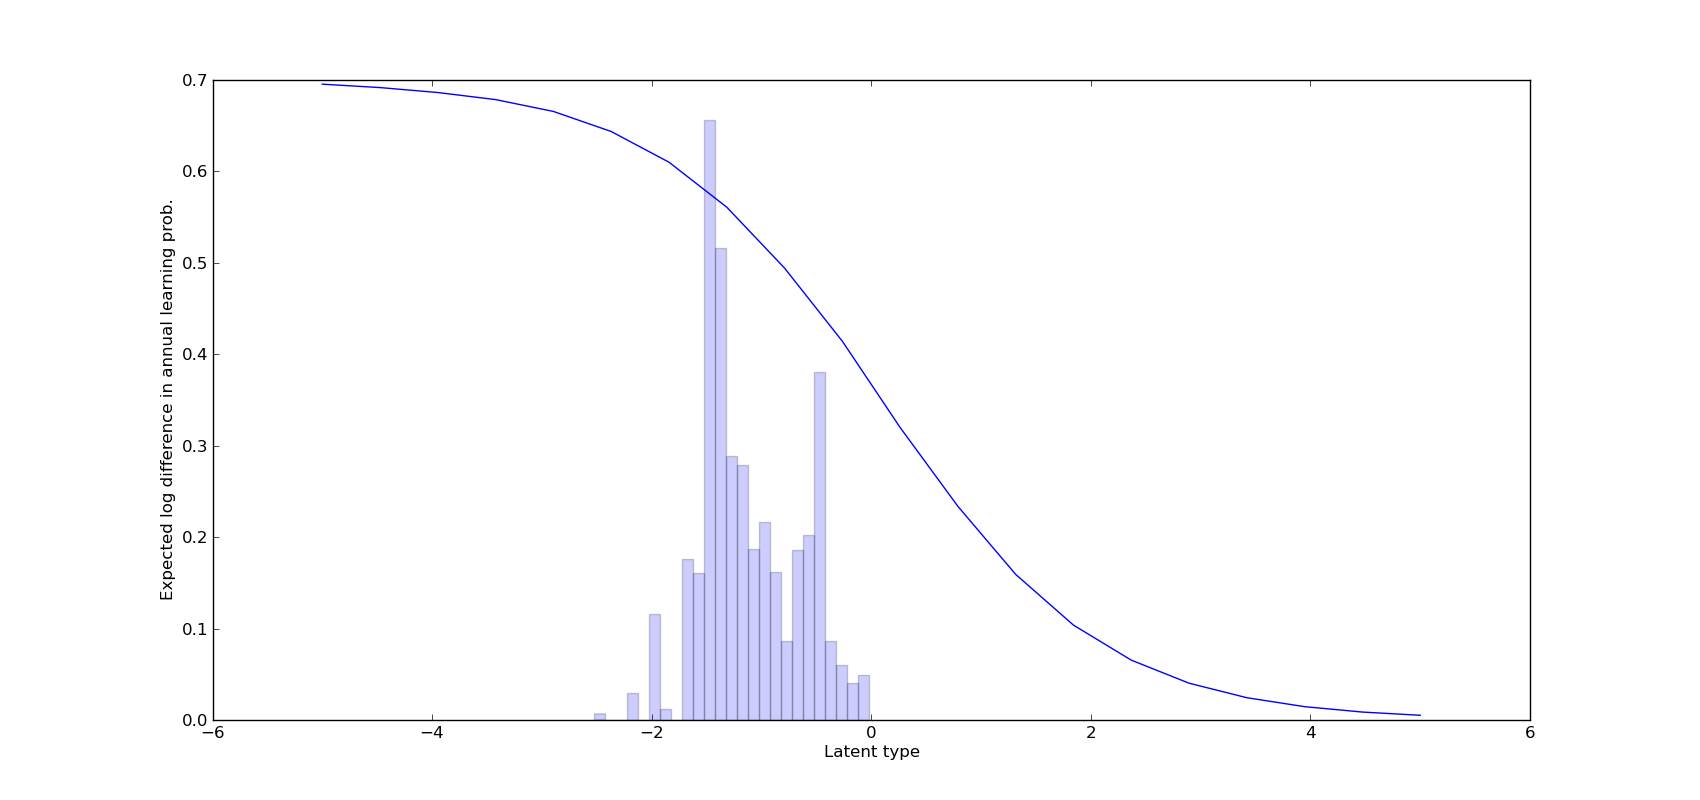
\includegraphics[scale=0.35]{pics/learn_probs.png}
    \caption{Annual learning probability percent increase, 0\% to 5\% coworker knowledge of new paper}
    \label{fig:learn_probs}
\end{figure}

The bottom two rows of Figure \ref{fig:big_params} contains posterior distributions for the
moving parameters. The field and quality wage
interaction coefficients $\xi$ have a positive sign in expectation, meaning
that we expect people to sort towards own type in both field and quality dimensions. The coefficient on the 
field interaction, 
however, is estimated without much precision and very well may be close
to zero or negative. The movement cost parameter is large relative to the wage interactions, providing a strong 
disincentive to moving.  The 1991 payoff effect $\xi_{ex}$ reflects the extent that
wages in affected states dropped to generate moving patterns in the
data. The mean value is
0.87, which implies that a public school in a state with a budget
shortfall of 10\% would see a 1991 payoff drop of about
$e^{-0.919 \times 0.1} \approx 9\%$.\footnotemark\footnotetext{The entry and exit processes
    of academics is not modeled here, and the size of economics departments has been growing
    rapidly over the last thirty years.  The model therefore has little to say about
    what distribution of academics over departments we should expect to see in the data.  Even so, Appendix
    \ref{sec:movdists} contains some discussion of the long-run distribution of academics
    across departments implied by the estimation results, and compares this distribution with what is
    observed in the data.}

The latent type distribution parameter posteriors are located in the bottom
row of Figure \ref{fig:big_params}. The first column relates to the initial
mean of the distribution of latent type $h_i$. $\phi_F$ and $\phi_Q$ are both negative, so that
a department with high field fraction and quality has lower average initial latent type values.  This result is consistent with
the sorting implied by the negative coefficient on the wage interaction between latent type and field $\xi_l$.
The standard deviation of latent type is estimated to be a bit less than one.

\subsection{Intuition for Counterfactuals}
\label{sec:count_int}

Before I get to the results of the counterfactual exercise, first I present some
intuition using a toy model.  The goal in this section is to show that we should expect
an increase in movement between departments to make them more similar in terms of knowledge fractions,
as well as increase aggregate diffusion.  Consider a simple continuous-time theoretical model of
diffusion. Let there be a single firm with a continuum of workers in
which there is a hazard of learning about a new idea given by:

\begin{equation}
    \lambda(t) = \alpha + \beta S(t)
\end{equation}

S(t) is the share of people in the firm who know about the new idea at
time $t$. As in the empirical model
developed above, it is easier to learn about a new paper as
more people come to know about it. Suppose that a new innovation is developed at time
zero. We can describe the evolution of $S$ by the 2nd-order differential
equation:

\begin{equation}
    \frac{dS(t)}{d t} = \left( \alpha + \beta S(t) \right) \left(1 - S(t)\right)
    \label{eq:difeq_orig}
\end{equation}

Solving for $S$ gives:

\begin{equation}
    S(t) = \frac{\alpha e^{\left(\alpha + \beta \right) t} - \alpha}{\alpha e^{\left(\alpha + \beta \right) t} + \beta}
    \label{eq:difeq}
\end{equation}

This is the logistic curve, which has long been used to model the spread
of innovations.

Now consider two symmetric firms in which the innovation is spreading
independently as above. If the firms are exactly the same, movement will
not have any effect on knowledge spread. Suppose instead that one firm,
the leading firm, gets a head start learning about the new innovation.
The second firm, the lagging firm, begins to learn about the innovation
only after some time. This situation is illustrated in Figure
\ref{fig:simp_dif}. The horizontal axis is time since the beginning of
learning about the innovation, and the vertical axis is share of people
who know about the new idea. The leading firm is farther up the logistic
diffusion curve.

\begin{figure}[!ht]
    \centering
    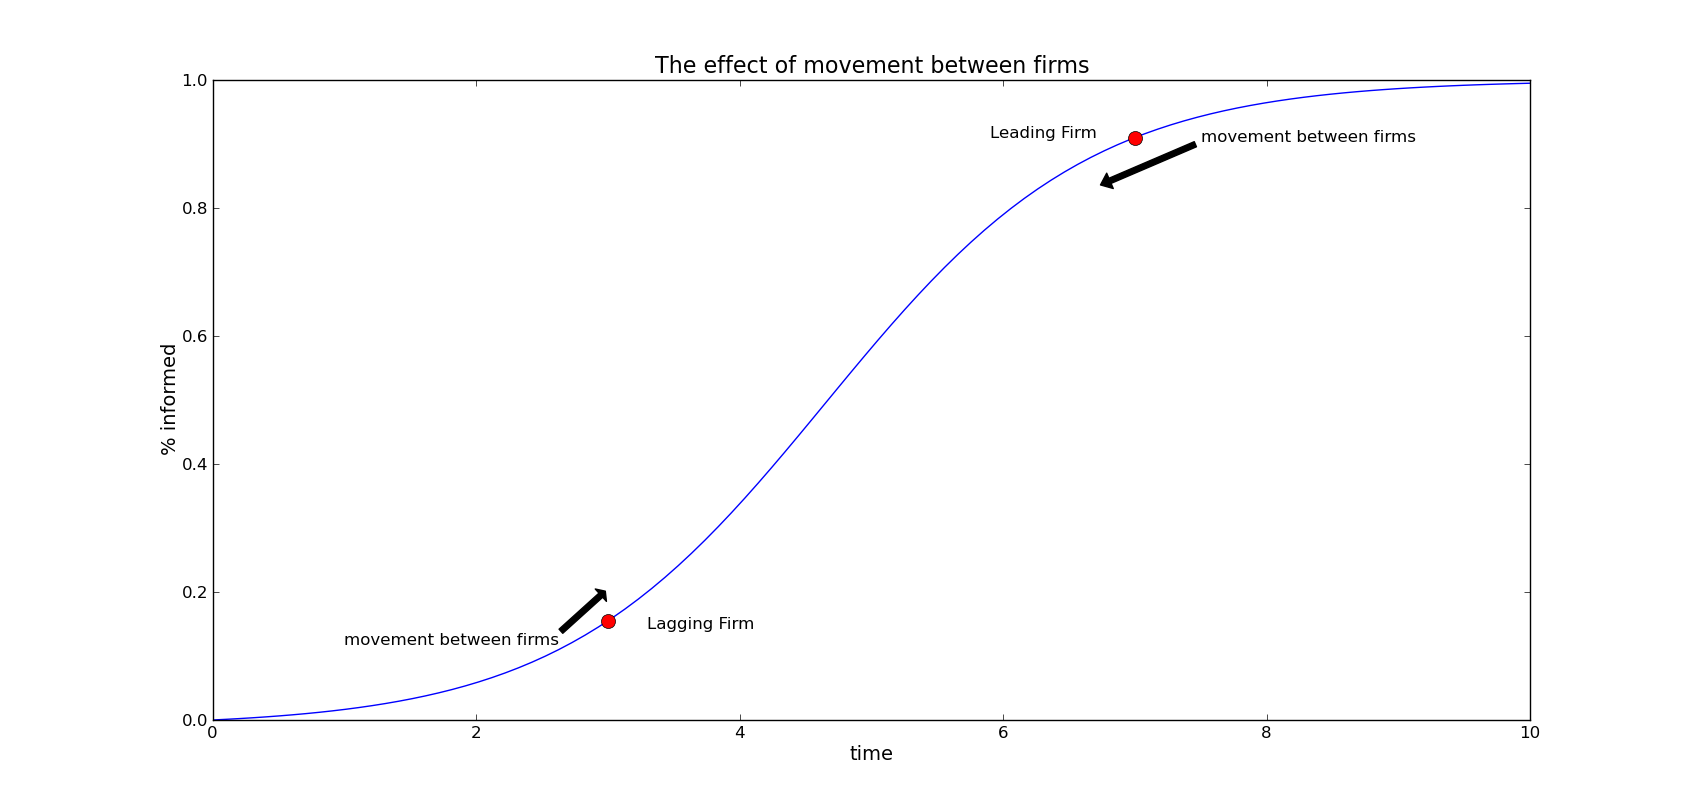
\includegraphics[scale=0.35]{plots/mean_field_logistic.png}
    \caption{Movement between firms on a diffusion curve}
    \label{fig:simp_dif}
\end{figure}

Randomly swap workers between firms. This will raise the share of people
in the lagging firm which know about the idea, and lower the share at
the leading firm, moving the two firms closer to each other on the
diffusion curve.  The steeper the section a firm is on, the
faster knowledge is diffusing within the firm. In the illustrated case
movement between firms will speed up diffusion because both firms will
be pulled onto a steeper part of the diffusion curve.

If both firms were on the initial convex part of the diffusion curve, however, one might 
expect that aggregate diffusion could be slowed down by movement.\footnotemark\footnotetext{An earlier draft of this paper made such an informal argument.} This is not so.
From \eqref{eq:difeq_orig}, the effect of an additional worker becoming informed on the rate of diffusion is given by:

\begin{equation}
\frac{d S'(t)}{d S(t)} = - \left( \alpha + \beta S(t) \right) + \beta \left(1 - S(t)\right)
\end{equation}

The first term on the RHS says that now there are less uniformed workers to learn the new idea, which slows the change in $S(t)$.  The second term says that the remaining uninformed workers are more likely to learn about the new idea, which increases the change in $S(t)$.  Suppose that a particular time the leading firm has $S(t) = s_h$ and the lagging firm has $S(t) = s_l$, with $s_h > s_l$.  Then the change in aggregate diffusion resulting from an informed-uninformed worker swap is given by:

\begin{equation}
- \left( \alpha + \beta s_l \right) + \left( \alpha + \beta s_h \right) + \beta \left(1 - s_l\right) - \beta \left(1 - s_h\right) = 2 \beta (s_h - s_l)
\end{equation}

This expression is positive, so the effect of marginal worker movement on aggregate diffusion is positive.  \footnotemark\footnotetext{If $\beta = 0$ so that learning does not depend on coworkers, then \eqref{eq:difeq} reduces to the exponential distribution. In this case, mixing between firms has no effect on the diffusion rate, as one would expect.  To see this, consider two firms both of size one, one at $t_1$ on the diffusion curve, and the other at $t_2$.  The aggregate diffusion rate is $z^* = \alpha e^{\alpha t_1} + \alpha e^{\alpha t_2}$.  Now combine the two firms.  The knowledge share at the combined firm is:

\begin{equation} 
    y^* = \frac{(1 - e^{-\alpha t_1}) + (1 - e^{-\alpha t_1})}{2} = 1 - \frac{z^*}{2\alpha} \nonumber
\end{equation}

Find the appropriate time argument associated with share $y^*$ on the diffusion curve:

\begin{align*}
    y^* &= 1 - e^{-\alpha t^*} \\
    1 - \frac{z^*}{2\alpha} &= 1 - e^{-\alpha t^*} \\
    t^* &= \frac{\ln (\frac{z^*}{2 \alpha})}{-\alpha} \\
\end{align*}

Finally get the new diffusion rate (the new firm has population two):

\begin{equation}
    2 \alpha e^{- \alpha t^*} = 2 \alpha e^{\ln (\frac{z^*}{2 \alpha})} = z^* \nonumber
\end{equation}

As expected, combining the firms has no effect on the aggregate diffusion rate.  The only way that movement can effect aggregate diffusion is through the dependence parameter $\beta$.}

Even though the model developed in this section is just a toy, the logic
goes through to the empirical model developed above. Movement between
firms should make firms both more similar in terms of knowledge shares and increase aggregate diffusion.
\subsection{Counterfactual Results}

The counterfactuals in this section involve varying the movement cost parameter $\mathcal{C}$. 
I begin  by drawing a set of parameters from the
estimated posterior distribution, and then simulate the model using the academics 
in my dataset and the ergodic distribution of academics over departments. I draw a
department, latent type, interest for each academic using the estimated
parameters. Results are generated for four values of
$\mathcal{C}$: the full estimated cost parameter, 70\% of the parameter, 50\% of the parameter, and totally shutting down the cost of moving between departments.  In the estimation data, about 3-4\% of academics move each year.  70\% of the cost parameter is chosen because it induces 9-10\% of academics to move each year.

\begin{figure}[!ht]
    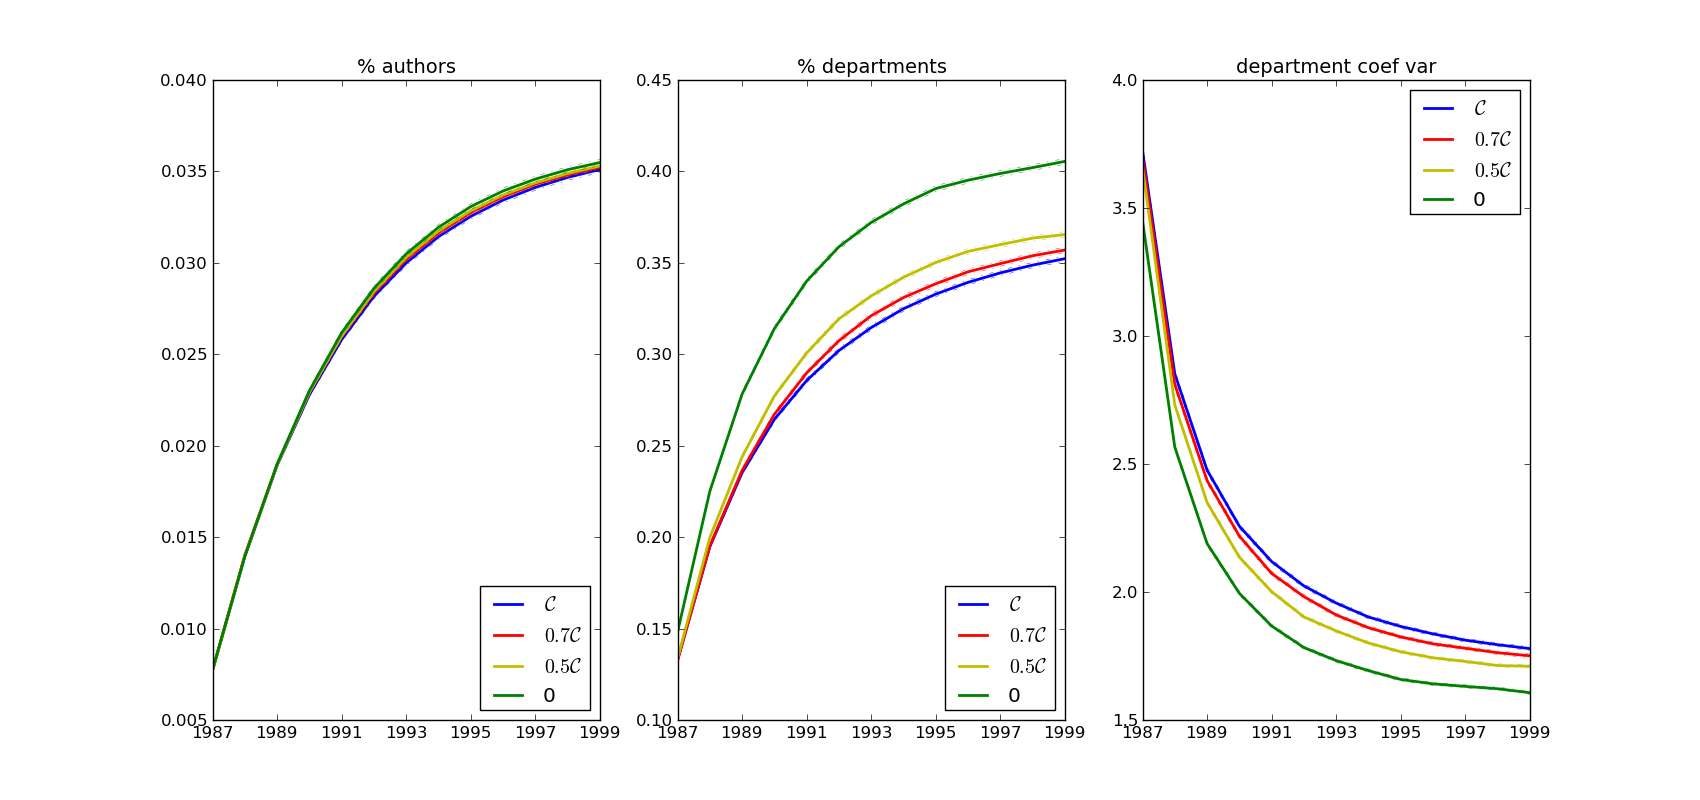
\includegraphics[scale=0.35]{pics/sim_plots_cf.png}
    \caption{Counterfactual statistics, posterior expectations}
    \label{fig:cf}
\end{figure}

We will focus on three statistics to characterize the generated data: the percentage of academics who
have cited the paper, the percentage of departments housing someone who cited the
paper, and the coefficient of variation over departments in fraction of members who
have cited the paper. Figure \ref{fig:cf} plots the expected evolution
of those three statistics in the different scenarios. Figure \ref{fig:cf_frac} plots
the posterior expectation of the log
difference between counterfactual statistics and simulated data statistics. The bottom row of Figure \ref{fig:cf_frac}
is the log difference between the data offer rate and half of the offer rate.  In both figures,
the dotted lines are the 90\% confidence intervals on the
expectation of the posterior distribution.

\begin{figure}[!ht]
    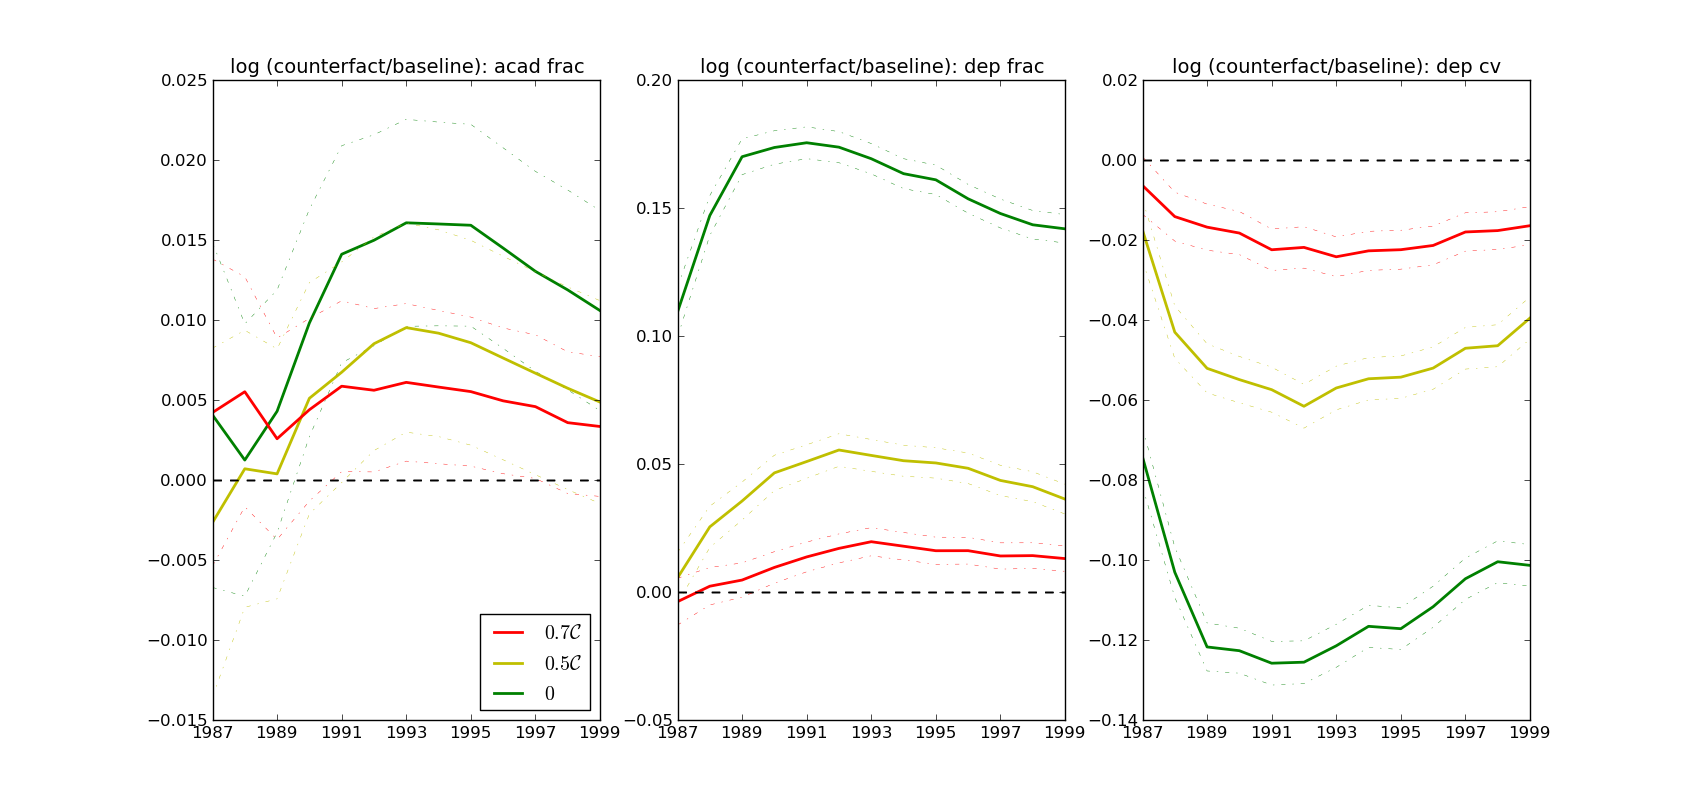
\includegraphics[scale=0.35]{pics/sim_plots_cf_frac.png}
    \caption{log change in posterior expectations}
    \label{fig:cf_frac}
\end{figure}

As expected, more mobility increases the fraction of departments employing at least one person who has
cited the paper, and the reduces variation in knowledge fractions between departments. 
If we compare the no cost to the benchmark
case, then within several years after the idea begins diffusing, we expect 15-20\% more
departments to house at least one person who knows about the paper.
Likewise, we expect a 12\% lower coefficient of variation between departments. 
The less dramatic counterfactuals push diffusion
 in the same direction, although the effects are smaller. We expect that 1.5\% more academics will have heard about a 
 new paper seven years after it is published in the no cost counterfactual. 

 All of the log difference plots exhibit a U shape because in the model ideas eventually diffuse completely.  
 As time goes to infinity, all potentially interested academics learn about the new paper. 
 As expected, increasing movement between departments speeds up knowledge diffusion.

\section{Extension to Cross-Country Diffusion}

This section calibrates a model of international knowledge diffusion using 
information from the estimated structural model.  In particular, I show that
a small increase in movement of Chinese academics between China and the United
States can significantly increase the diffusion of foreign knowledge in China.
In recent years, Chinese scholars have been spending more time as visitors in 
the United States.  In my time at Penn State, our department has housed several
visiting Chinese researchers, and a faculty member told me that he frequently receives 
emails from Chinese economists asking to pay their own way to visit.

As mentioned above, an academic only appears in my data when he
publishes in one of the journals tracked by the Web of Knowledge.  The
data is very sparse for China and other developing countries.  Using outside data,
I calibrate the structure of the Chinese 
academic labor market.  I assume that the 117 participating universities in
a Chinese government program for improving higher education make up the universe
of active research universities.\footnotemark\footnotetext{I am referring to the 221 Program.
    For more information on this program see \citet{lixu2004china}.  I found the 
list of universities on Wikipedia.}
   Based on my impression from clicking through 
department websites, I further assume that each department has on average
twenty active research faculty.  Since I have no information on department or academic 
quality or field, I assume that departments and academics are homogeneous.

As in the United States, I model academics in China moving between departments,
and learning about new papers.  Since departments and academics are 
homogeneous, moves are random.  I assume that each Chinese academic has a 2.2\%
chance of changing his domestic affiliation each year, matching the observed 
movement rate in the American data.

The probability of learning about a new paper in China is still given by
\eqref{eq:citprob}, but with different parameter values than in the United
States:  

\begin{equation}
    \frac{e^{\alpha_c + \beta_c K(d,t-1) + h_i}}{1 + e^{\alpha_c + \beta_c K(d,t-1) + h_i}}
    \label{eq:citprob_china}
\end{equation}

As Chinese moves are random, for simplicity I will assume that all Chinese academics
have the same latent type equal to the average latent type
of Americans.  The first Chinese citation of the Jensen paper in my data is
from Hong Kong in 1995, and then from mainland China in 1997.  Assuming that 
Chinese academics have the same probability of interest in the Jensen paper
as American academics not in Jensen's field ($\gamma_c = \gamma_0$), I set the Chinese base learning 
hazard $\alpha_c$ so that the first cite is expected nine years after publication.
I calibrate the Chinese dependent hazard $\beta_c$ so that the increase in
learning probability from no coworker knowledge of a new paper to 5\% is the same
as in the estimated domestic structural model for the average latent type.\footnotemark\footnotetext{
To be clear, I set $\alpha_c$ to satisfy:

\begin{equation}
    \frac{1}{9} = \alpha_c * \gamma_c * \vert A_c \vert
\end{equation}

Here $\vert A_c \vert$ is the number of Chinese academics.  I set $\beta_c$
 to satisfy the following equality:

\begin{equation}
    \frac{e^{\alpha + \beta 0.05 + \bar{h}}}{1 + e^{\alpha + \beta 0.05 + \bar{h}}} - \frac{e^{\alpha + \bar{h}}}{1 + e^{\alpha + \bar{h}}} = \frac{e^{\alpha_c + \beta_c 0.05 + \bar{h}}}{1 + e^{\alpha_c + \beta_c 0.05 + \bar{h}}} - \frac{e^{\alpha_c + \bar{h}}}{1 + e^{\alpha_c + \bar{h}}}
\end{equation}
}

Everything related to American academics works exactly as in the domestic structural
model.  New in this model is international movement of
Chinese academics.  With annual probability $\lambda_c$, a Chinese academic visits a random
American department for one year.  While in the United States, a potentially interested
visitor will learn about the new paper with the American probability \eqref{eq:citprob}.  I
simulate the model with three values of $\lambda_c$: 0, 0.01, and 0.02, and
1100 random draws of parameters from the posterior distribution.

\begin{figure}[!ht]
    \centering
    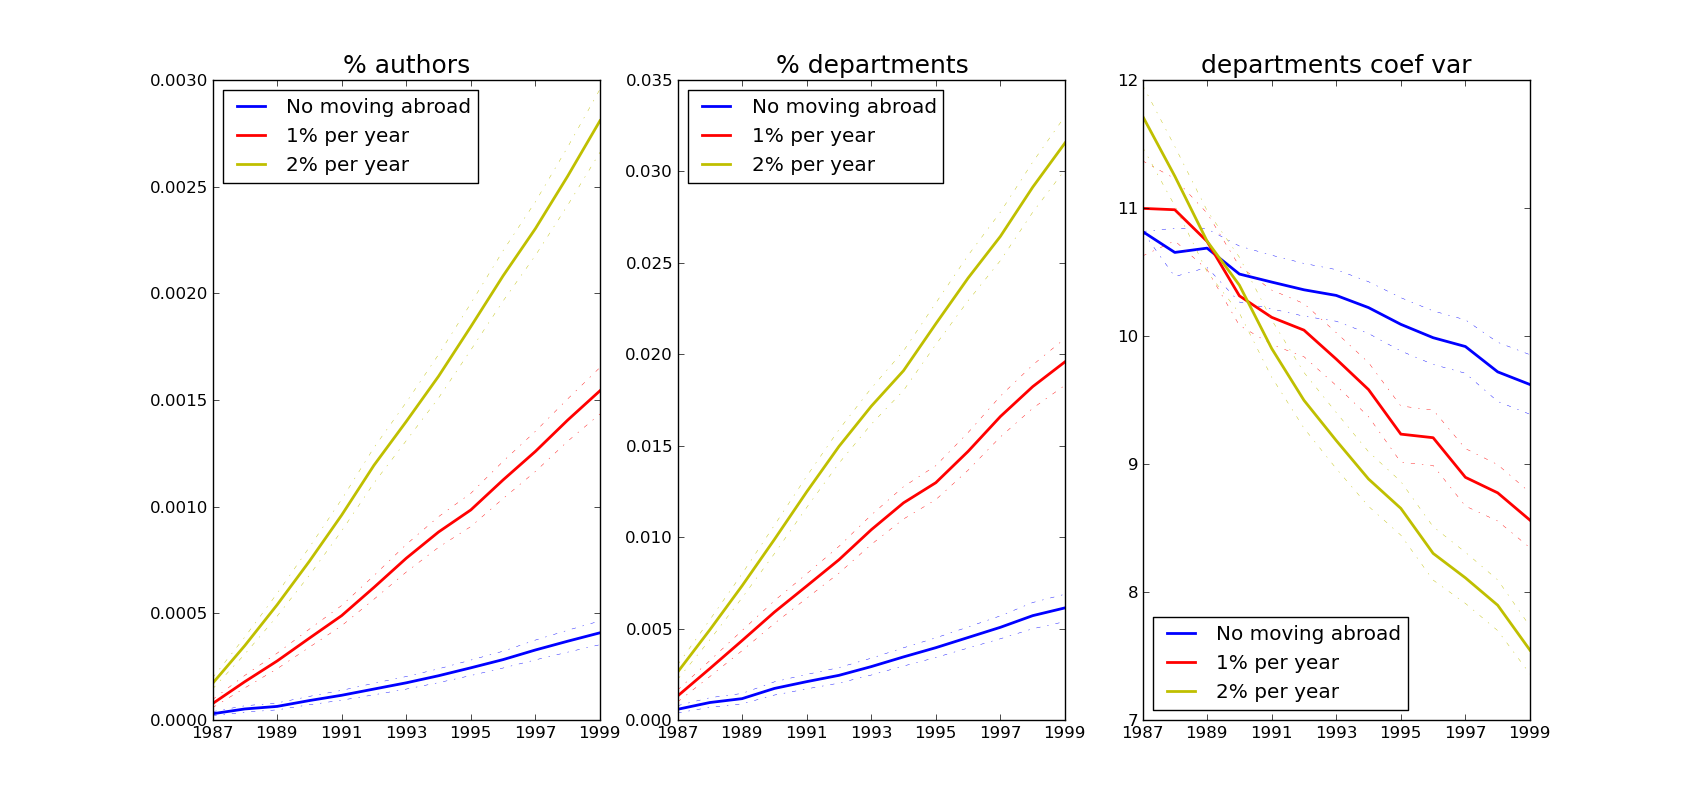
\includegraphics[scale=0.35]{pics/sim_plots_cs.png}
    \caption{Expected Chinese knowledge diffusion}
    \label{fig:chinsim}
\end{figure}

Figure \ref{fig:chinsim} plots for China the expected evolution of the three 
statistics we focused on in the counterfactual section above: the percentage of academics
who know about the paper, the percentage of departments housing at least one academic 
who knows about the paper, and the coefficient of variation over departments in fraction 
of informed academics.  International exchange
 directly increases the fraction of informed Chinese academics because it is
 easier to learn about the new paper abroad.  There is a slight convexity in the 
left-hand panel plotting the percentage of Chinese academics who have learned about
the paper by a given year.
There are two causes for the convexity.  The first is that it is getting easier 
over time to learn about the paper in the United States, so an academic is more likely
to learn while visiting abroad.  This effect dies after the first few years because
knowledge about the paper spreads quickly in the United States.  Secondary transmission
causes the convexity of the line in later years.  It is hard
to discover a new American paper alone in China, but the knowledge of coworkers greatly
facilitates learning.

The calibration contained in this section is rough and suggestive, but it underlines an important
 direction for future research.  Past research has pointed to large welfare gains from
reduction in barriers to migration.\citep{clemens2011economics}  Typically this
 line of research does not consider migrants as vectors for technology diffusion.  If migrants 
can move knowledge between places, then not only will welfare gains to additional
migration be larger than the previous literature has estimated, but distribution of welfare gains 
will change as source country workers benefit from the knowledge
of return migrants.  More rigorous estimation of international labor movement and
 knowledge diffusion is a natural next step in this project.

\section{Alternative Model Specifications}
\label{sec:extensions}

In this section, three extensions to the basic structural model are
presented. In the first extension, I add a national dependent probability
to the learning specification \eqref{eq:citprob} above. This model
captures a time effect.  As more people learn about a new idea, an academic is more likely to run into
someone who knows about the idea at a conference or seminar. This model weakens the importance of location,
as anyone learning about the paper anywhere increases learning probabilities for all other academics.  In
\eqref{eq:citprob_reg}, $K(n,t-1)$ is the aggregate percentage of academics who cited the paper by $t-1$.

\begin{equation}
    \frac{e^{\alpha + \beta K(d,t-1) + \beta_n K(n,t-1) + h_i}}{1 + e^{\alpha + \beta K(d,t-1) + \beta_n K(n,t-1) + h_i}}
    \label{eq:citprob_reg}
\end{equation}

In a second extension, the diffusion process parameters are all allowed
to depend on field. That is, if an academic is in the Jensen field, we rewrite
\eqref{eq:citprob} all with $f$ subscripts as in \eqref{eq:citprob_field}.

\begin{equation}
    \frac{e^{\alpha_f + \beta_f K(d,t-1) + h_i}}{1 + e^{\alpha_f + \beta_f K(d,t-1) + h_i}}
    \label{eq:citprob_field}
\end{equation}

The last extension is a simple publication lag.  I assume that if we observe a cite in, say, 1991,
the academic actually learned about the paper in 1990.  To maintain comparability with the other model
specifications, I maintain the assumption that an academic cannot learn about the Jensen paper
until 1987, the year after it was published.  To estimate the publication lag extension,
I pool the three observed 1987 cites in with the observed 1988 cites.

\begin{table}[!ht]
    \centering
    \begin{tabular}{lllllllll}
        \hline\hline;
       \textbf{param} & \multicolumn{2}{c}{\textbf{baseline}} & \multicolumn{2}{c}{\textbf{field-dep}} & \multicolumn{2}{c}{\textbf{nation}}  & \multicolumn{2}{c}{\textbf{lag}}    \\ \hline 
        $\alpha$      & -0.447 & (0.179) & -0.574 & (0.204) & -0.955 & (0.184) & -0.252 & (0.159) \\ 
        $\alpha_f$    &        &         & 0.170  & (0.488) &        &         &        &         \\ 
        $\beta$       & 14.128 & (5.850) & 16.991 & (5.881) & 6.537  & (4.654) & 10.418 & (4.295) \\ 
        $\beta_f$     &        &         & 78.846 & (71.576)&        &         &        &         \\ 
        $\beta_n$     &        &         &        &         & 81.257 & (16.031)&        &         \\ 
        $\gamma_{nf}$ & 0.035  & (0.004) & 0.036  & (0.005) & 0.027  & (0.003) & 0.028  & (0.003) \\ 
        $\gamma_{f}$  & 0.094  & (0.031) & 0.078  & (0.032) & 0.071  & (0.022) & 0.084  & (0.026) \\ 
        $\xi_f$       & 2.208  & (1.374) & 2.310  & (1.379) & 2.347  & (1.434) & 2.302  & (1.379) \\ 
        $\xi_l$       & -0.293 & (0.411) & -0.269 & (0.425) & -0.082 & (0.421) & -0.095 & (0.423) \\ 
        $\xi_q$       & 1.050  & (0.021) & 1.051  & (0.020) & 1.084  & (0.019) & 1.084  & (0.018) \\ 
        $\phi_Q$      & -1.302 & (0.014) & -1.302 & (0.017) & -1.297 & (0.015) & -1.298 & (0.016) \\ 
        $\phi_F$      & -7.603 & (0.230) & -7.627 & (0.265) & -7.629 & (0.224) & -7.606 & (0.234) \\ 
        $\sigma$      & 0.499  & (0.005) & 0.499  & (0.005) & 0.496  & (0.005) & 0.496  & (0.005) \\ 
        $\mathcal{C}$ & 8.426  & (0.052) & 8.425  & (0.049) & 8.651  & (0.049) & 8.655  & (0.049) \\ 
        $\xi_{ex}$    & 0.919  & (0.739) & 0.001  & (0.026) & 0.095  & (0.282) & 0.082  & (0.245) \\ \hline
    \end{tabular}
    \caption{Posterior expectations, extensions versus baseline}
    \label{tab:ext_post}
\end{table}

%Reset footnote counter
\setcounter{footnote}{0}

Priors are the same relatively uninformative priors used in the baseline model.  Table \ref{tab:ext_post} compares the expectations of posteriors for the baseline model and extensions.\footnotemark\footnotetext{Estimated posterior kernel densities 
    for all extensions can be found in Appendix \ref{sec:altmodels}.}
In the all extensions, the movement related parameters at the bottom of Table \ref{tab:ext_post} are
similar to those in the baseline model.

First consider the national dependence specification.
The department level $\beta$ is about half of the size of that
estimated in the baseline model, and the national parameter $\beta_n$ is large.
The national $\beta_n$ is, of course, multiplied by very small numbers since relatively few people ever
cite the Jensen paper overall.  The posterior for interest levels $\gamma$ and base learning parameter
$\alpha$ are similar to those in the baseline model.

As for the field-specific parameter model, the posteriors for those
not in the Jensen field are similar to the baseline model. 
relatively small sample size causes the
parameters for those in Jensen's field to be estimated with less
accuracy. The base learning parameter
$\alpha$ and the dependent learning parameter $\beta$  are both higher for those in the field.

The publication lag extension looks fairly similar to the baseline model.  The dependent learning parameter $\beta$ is a bit lower than in the baseline, and the base learning parameter  $\alpha$ is a bit higher.  This is due to the model trying to match the larger number of 1987 citers.  Since there is no colleague knowledge at that point, base learning must be ratcheted up to rationalize learning.

\subsection{Model Checking}
\label{sec:modcheck}

This section uses the baseline model as well as the three extensions to
simulate data, and then compares statistics of the simulated data to
the same statistics of the observed data. We will check the models on same
three dimensions: the diffusion of citations among academics, the
diffusion of citations between departments, and the coefficient of
variation across departments of percentage of academics who have cited the
paper. For each exercise, 2000 vectors of parameter values are drawn
from the posterior distributions, and the model is simulated at each parameter value.
The movement posteriors in the regional and field dependence extensions are
nearly identical to those in the baseline model.
In order to increase computation speed, we simulate moves out of the
baseline model, and then simulate idea diffusion using the baseline and extended
models separately.  Both moves and citation times are simulated separately for
the publication lag model.

\begin{figure}[!ht]
    \centering
    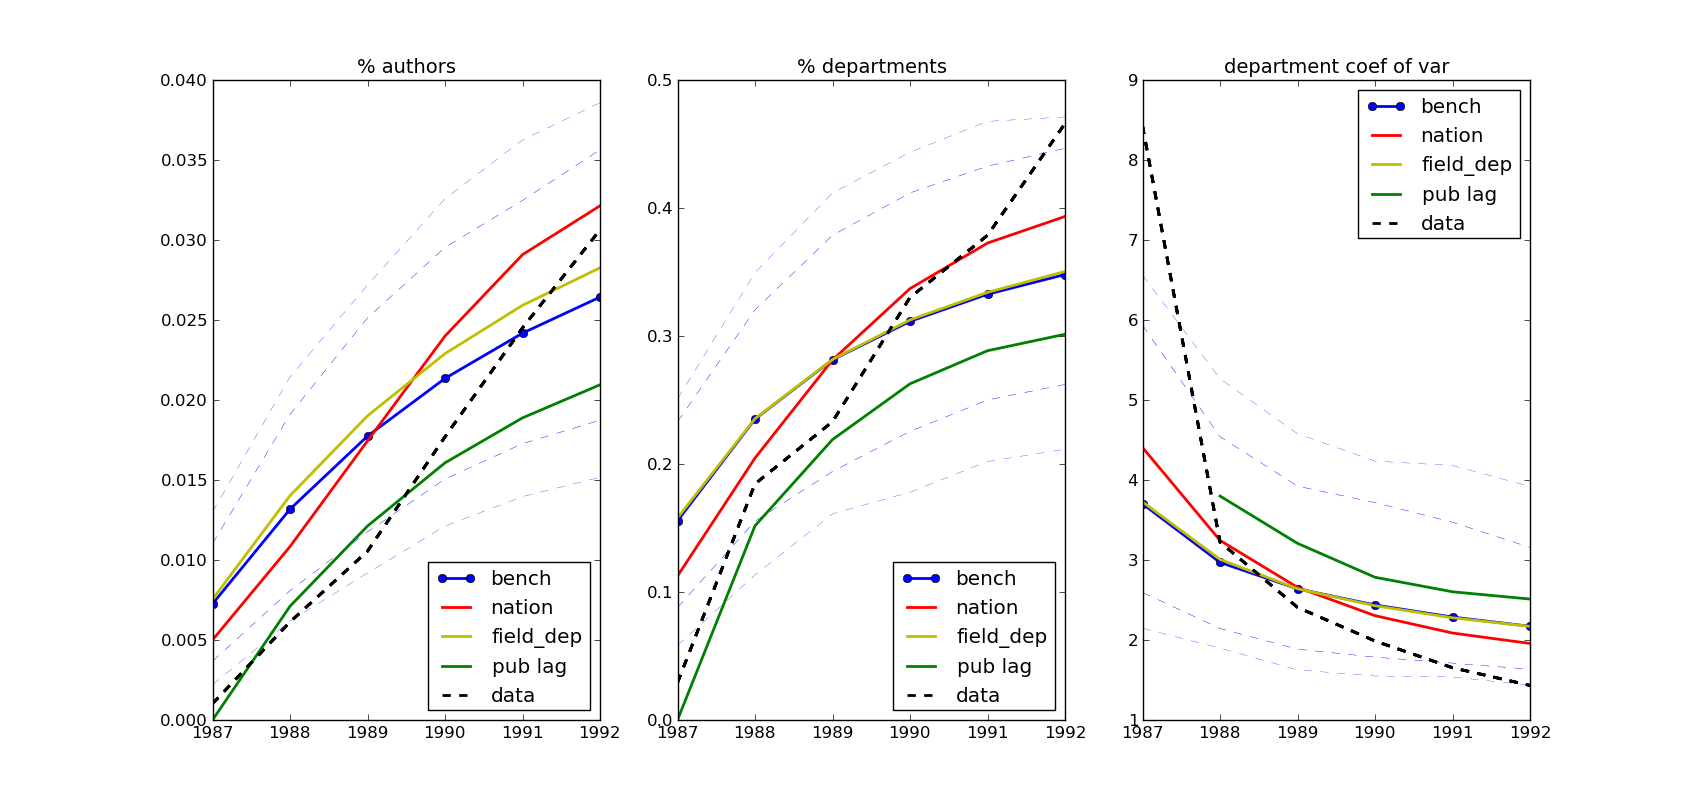
\includegraphics[scale=0.35]{pics/sim_plots_mc.png}
    \caption{Model checking, simulations vs data}
    \label{fig:modcheck}
\end{figure}

Figure \ref{fig:modcheck} contains posterior means for the three model
scenarios and data.  When interpreting this exercise, the reader should keep
in mind that we are comparing means of many simulations to the data, which should
be thought of as a single random realization.  We have only 122 first citations in 
the data, and most of these come toward the end of the data period. There is sizable 
random variation in the simulated trajectories.  To make this point, the
95\% and 99\% credible intervals of the baseline model are included
as faint lines in Figure \ref{fig:modcheck}.  Save for the first year, the data
is always within the 99\% credible interval of the baseline model.

Except for the publication lag model, all models overestimate the number
of citers in the first year in the raw data. In the raw data, there are
only three citing academics in the first year.  As time goes by, the levels
in the data and in the models become more similar.  Of the three models,
the publication lag model does the best in the first few years, but misses
the data in the final years.  The national dependence model fits the qualitative
slope of the data the best, but its level is too high for the entire
simulation period.  The benchmark and field-specific
parameter models display very similar behavior, and are generally in between
the baseline and the publication lag model in level.

\section{Instrumented Probit Model}
\label{sec:end_probit}

\begin{table}[!ht]
    \centering
    \begin{tabular}{lllllll}
    \hline\hline
                        &       cit92   &       cit92   &       cit92   &    cit92\_93  &    cit92\_93  &    cit92\_93  \\
                        &        b/se   &        b/se   &        b/se   &        b/se   &        b/se   &        b/se   \\
    \textbf{probit eq 1}&               &               &               &               &               &               \\ \hline
            kfrac       &      26.952*  &      37.604*  &      40.753** &      26.362** &      38.034** &      41.238** \\
                        &     (14.78)   &     (19.84)   &     (16.95)   &     (11.68)   &     (15.97)   &     (18.75)   \\
              field     &               &       0.000   &       0.000   &               &       0.023   &       0.029   \\
                        &               &         (.)   &         (.)   &               &      (0.18)   &      (0.12)   \\
            qual        &               &       0.001   &       0.001   &               &       0.001   &       0.001   \\
                        &               &      (0.00)   &      (0.00)   &               &      (0.00)   &      (0.00)   \\
            dep\_qual   &               &      -0.048   &      -0.053   &               &      -0.052*  &      -0.070*  \\
                        &               &      (0.04)   &      (0.04)   &               &      (0.03)   &      (0.04)   \\
            dep\_field  &               &       1.996   &       1.275   &               &       1.366   &       1.151   \\
                        &               &      (4.21)   &      (5.64)   &               &      (3.22)   &      (4.58)   \\
            public      &               &               &       0.060   &               &               &      -0.010   \\
                        &               &               &      (0.30)   &               &               &      (0.32)   \\
            dep\_size   &               &               &               &               &               &       0.006   \\
                        &               &               &               &               &               &      (0.01)   \\
            \_cons      &      -2.513***&      -1.012   &      -0.491   &      -2.319***&      -0.735   &      -0.277   \\
                        &      (0.64)   &      (2.77)   &      (3.84)   &      (0.47)   &      (2.08)   &      (3.65)   \\ \hline \hline
    \textbf{probit eq 2}&      kfrac    &      kfrac    &      kfrac    &      kfrac    &      kfrac    &      kfrac    \\ \hline
            bd          &      -0.061***&      -0.023   &      -0.014   &      -0.061***&      -0.023   &      -0.011   \\
                        &      (0.01)   &      (0.05)   &      (0.06)   &      (0.01)   &      (0.05)   &      (0.06)   \\
              field     &               &       0.000   &       0.000   &               &      -0.001   &      -0.001   \\
                        &               &         (.)   &         (.)   &               &      (0.00)   &      (0.00)   \\
            qual        &               &      -0.000   &      -0.000   &               &      -0.000*  &      -0.000*  \\
                        &               &      (0.00)   &      (0.00)   &               &      (0.00)   &      (0.00)   \\
            dep\_qual   &               &       0.001***&       0.001***&               &       0.001***&       0.002***\\
                        &               &      (0.00)   &      (0.00)   &               &      (0.00)   &      (0.00)   \\
         dep\_field     &               &      -0.005   &      -0.004   &               &      -0.005   &      -0.011   \\
                        &               &      (0.08)   &      (0.08)   &               &      (0.08)   &      (0.08)   \\
            public      &               &               &      -0.001   &               &               &      -0.000   \\
                        &               &               &      (0.01)   &               &               &      (0.01)   \\
            dep\_size   &               &               &               &               &               &      -0.000   \\
                        &               &               &               &               &               &      (0.00)   \\
            \_cons      &       0.024***&      -0.009   &      -0.008   &       0.024***&      -0.010   &      -0.009   \\
                        &      (0.00)   &      (0.01)   &      (0.01)   &      (0.00)   &      (0.01)   &      (0.01)   \\ \hline
            CD Wald F   &      31.41    &        5.66   &        0.74   &        16.38  &        5.66   &        0.74   \\ \hline
            obs         &      2940     &        2845   &        2845   &        2940   &       2940    &       2940    \\ \hline

    \end{tabular}
    \caption{Probit model}
    \label{tab:endprob}
\end{table}

This section estimates an alternative reduced-form model for
knowledge diffusion.  The probit model developed here is for citing in 1992, and uses
1991 budget deficits as an instrument for knowledge fractions.  The idea is that budget cuts
affect movement and substitution patterns across departments.  To give an example, suppose that Berkeley 
was planning on hiring a junior faculty member in contract theory in 1991, but couldn't because 
there was a hiring freeze.  The junior contract theorist who had already cited Jensen's paper and would 
have gone to Berkeley instead went to NYU.  The exogeneity
condition is that a budget cut only affects citation probability through its 
affect on knowledge fractions at departments.
Let $C^{1992}_i$ be a dummy which
is one if academic $i$ cited the Jensen paper for the first time in 1992,
let $\mathbf{X}_{o,i}$ be a vector of observed characteristics, let $b_{d,i}$ be the
budget shortfall in the state of the (public university) department in
which academic $i$ worked in 1991, and let $K_i$, the knowledge fraction,
be the fraction of coworkers who have cited Jensen before 1992. The
observations are all academics who have not cited the Jensen paper as of
1992. The natural probit specification is:

\begin{equation}
    C^{1992}_i = 1_{\{ \beta_X \mathbf{X}_{o,i} + \beta_K K_i + \varepsilon_i > 0\}}
\end{equation}

And:

\begin{equation}
    K_i = \Gamma_X \mathbf{X}_{o,i} + \Gamma_{b_d} b_{d,i} + v_i
\end{equation}

Here we assume that $v_i$ and $\varepsilon_i$ are jointly normal and
correlated. I estimate the probit twice using the ivprobit function in
STATA, once using 1992 citers as described above and once assuming the
budget deficit effect lasted for two years, with the dependent variable
being a dummy for either a 1992 or a 1993 first cite. The
right-hand-side variables are the 1991 analogues of the quantities in
the structural model. Field is a dummy which is one if an academic has the
field of contract theory or business economics. Department field
fraction is the mean field value of academics in the department in 1991.
Quality is mean lifetime citations per paper, and department quality is
the mean quality in the department in 1991. Department size is just the
number of authors in the department in 1991, and public is a dummy for
public universities. 


The probit results are contained in Table \ref{tab:endprob}.  Field is
omitted in the second and third models
because it is a perfect predictor of not citing for the first time in
1991. Department size is omitted in the third model because the
likelihood would not converge with it included. All standard errors are 
clustered at the department level.  The direction of the
kfrac ($K_i$) coefficient is significant and in the expected direction
in all models. Some of the Cragg-Donald F Statistics are lower than ideal.
The rule of thumb from \citet{staiger1997instrumental} is that this statistic
should be greater than ten.  The instrument may be weak in some specifications.
A back of the envelope calculation using the models with
only $K_i$ indicates that if 5\% of coworkers know
about a new paper rather than 0\% of coworkers, citing probability is higher 
by about $\Phi(-1.15) - \Phi(-2.5) \approx 12\%$.  Appendix \ref{sec:add_evid}
 contains two additional reduced-form exercises which provide
 evidence on the importance of location on knowledge diffusion.

\section{Summary}

This paper develops a model of movement and the diffusion of knowledge
between firms. The model is estimated on data from a panel of academics
and the diffusion citations. Both the main structural model and
a reduced-form exercises show that physical proximity facilitates learning
 about a new idea. In a counterfactual section, I find that increased worker mobility
 speeds the diffusion of knowledge between locations, reduces 
the dispersion in fraction of informed workers across firms, and has a
positive effect on the total diffusion of ideas across workers.
In a calibrated exercise describing Chinese scholarly visits to the United
States, I find that the international movement of workers can have a large 
effect on domestic idea diffusion in a developing country.

There are several directions in which to develop this research.  One is to examine the effect of the internet on the diffusion of ideas.  My data span the early 1980's when there was no internet to the present.  The speed at which citations diffuse in the data should be informative about how the internet has affected idea diffusion.  A second and stickier direction is to explicitly model serially correlated shocks which affect both sorting and citing.  Recent research by \citet{arcidiacono2011conditional} in estimating dynamic discrete choice models with serially correlated, unobserved state variables might prove useful for such an exercise.  Finally, as mentioned in the section on Chinese migration, using a similar model to rigorously estimate the effect of labor migration on international technology diffusion is a natural next step.
